\documentclass[bigchapter,type=bsc,colorback,accentcolor=tud1b]{tudthesis}
%tud1b ist das KOM-blau
%tud0b ist das grau aus der vorlage
%,twoside

%--------------------------------------------------------
% shows reference keys
%--------------------------------------------------------
%TODO: remove for final
%\usepackage{showkeys}

%--------------------------------------------------------
% provides the todo command
%--------------------------------------------------------
\newcommand\todob[1]{{\color{red}\fbox{
\begin{minipage}{\textwidth-4pt}\texttt{ TODO: #1 }\end{minipage}}}}

\newcommand\todo[1]{{\color{red}\fbox{\texttt{\footnotesize TODO: #1}}}}

%--------------------------------------------------------
% more package references
%--------------------------------------------------------
%\usepackage{ngerman}   ...ist ja gar nicht auf deutsch!
\usepackage{booktabs}
\usepackage{tabularx}

\usepackage{hyperref}

\usepackage{varwidth}

\usepackage{graphicx}
\usepackage{wrapfig}
\usepackage{float}

\usepackage[bibencoding=utf8,style=alphabetic,sorting=anyt]{biblatex}
%\usepackage{parskip}

% new page for each section
%\usepackage{titlesec}
%\newcommand{\sectionbreak}{\clearpage}

% flow charts etc.
\usepackage{tikz}
\usetikzlibrary{shapes,arrows,positioning,automata}

\usepackage{listings}
\usepackage{lstlinebgrd}

\usepackage[toc,page]{appendix}


\usepackage{caption}
\usepackage{subcaption}


%--------------------------------------------------------
% configuration
%--------------------------------------------------------

%\bibliographystyle{IEEEtran}
\bibliography{thesis-h2-mptcp}

\setlength{\parskip}{0.75\baselineskip}%
%\setlength{\parindent}{0pt}%

% increase line height
\renewcommand{\baselinestretch}{1.2} 

\newcommand\code[1]{\texttt{\protect\detokenize{#1}}}

% german month for TUDthesis
\newcommand{\getmydate}{%
	\ifcase\month%
	\or Januar\or Februar\or M\"arz%
	\or April\or Mai\or Juni\or Juli%
	\or August\or September\or Oktober%
	\or November\or Dezember%
	\fi\ \number\year%
}

\definecolor{mygreen}{rgb}{0,0.6,0}
\definecolor{mygray}{rgb}{0.5,0.5,0.5}
\definecolor{mymauve}{rgb}{0.58,0,0.82}

\lstset{ %
  basicstyle=\footnotesize\ttfamily,        % the size of the fonts that are used for the code
  breakatwhitespace=false,         % sets if automatic breaks should only happen at whitespace
  breaklines=true,                 % sets automatic line breaking
  captionpos=b,                    % sets the caption-position to bottom
  commentstyle=\color{mygreen},    % comment style
  extendedchars=true,              % lets you use non-ASCII characters; for 8-bits encodings only, does not work with UTF-8
  frame=single,	                   % adds a frame around the code
  keepspaces=true,                 % keeps spaces in text, useful for keeping indentation of code (possibly needs columns=flexible)
  keywordstyle=\color{blue},       % keyword style
  %numbers=left,                    % where to put the line-numbers; possible values are (none, left, right)
  %numbersep=5pt,                   % how far the line-numbers are from the code
  %numberstyle=\tiny\color{mygray}, % the style that is used for the line-numbers
  rulecolor=\color{black},         % if not set, the frame-color may be changed on line-breaks within not-black text (e.g. comments (green here))
  showspaces=false,                % show spaces everywhere adding particular underscores; it overrides 'showstringspaces'
  showstringspaces=false,          % underline spaces within strings only
  showtabs=false,                  % show tabs within strings adding particular underscores
  %stepnumber=2,                    % the step between two line-numbers. If it's 1, each line will be numbered
  stringstyle=\color{mymauve},     % string literal style
  tabsize=2,	                   % sets default tabsize to 2 spaces
  title=\lstname                   % show the filename of files included with \lstinputlisting; also try caption instead of title
}
\lstdefinestyle{RBS}{
  language=C,                 % the language of the code
  morekeywords={SCHEDULER,VAR,IF,ELSE,FOREACH,RETURN,SET,IN}           % if you want to add more keywords to the set
}

\lstdefinestyle{C_Code}{
  language=C                 % the language of the code
}


\makeatletter
%%%%%%%%%%%%%%%%%%%%%%%%%%%%%%%%%%%%%%%%%%%%%%%%%%%%%%%%%%%%%%%%%%%%%%%%%%%%%%
%
% \btIfInRange{number}{range list}{TRUE}{FALSE}
%
% Test in int number <number> is element of a (comma separated) list of ranges
% (such as: {1,3-5,7,10-12,14}) and processes <TRUE> or <FALSE> respectively

\newcount\bt@rangea
\newcount\bt@rangeb

\newcommand\btIfInRange[2]{%
    \global\let\bt@inrange\@secondoftwo%
    \edef\bt@rangelist{#2}%
    \foreach \range in \bt@rangelist {%
        \afterassignment\bt@getrangeb%
        \bt@rangea=0\range\relax%
        \pgfmathtruncatemacro\result{ ( #1 >= \bt@rangea) && (#1 <= \bt@rangeb) }%
        \ifnum\result=1\relax%
            \breakforeach%
            \global\let\bt@inrange\@firstoftwo%
        \fi%
    }%
    \bt@inrange%
}
\newcommand\bt@getrangeb{%
    \@ifnextchar\relax%
        {\bt@rangeb=\bt@rangea}%
        {\@getrangeb}%
}
\def\@getrangeb-#1\relax{%
    \ifx\relax#1\relax%
        \bt@rangeb=100000%   \maxdimen is too large for pgfmath
    \else%
        \bt@rangeb=#1\relax%
    \fi%
}


%%%%%%%%%%%%%%%%%%%%%%%%%%%%%%%%%%%%%%%%%%%%%%%%%%%%%%%%%%%%%%%%%%%%%%%%%%%%%%
%
% \lstHighlightRange{range list}
%
% Highlights lines in range list in a lstlisting linebackgroundcolor parameter
\definecolor{codehladded}{HTML}{EAFFEA}
\definecolor{codehlremoved}{HTML}{FFECEC}
\definecolor{codehlhighlight}{HTML}{FFF9E8}

\newcommand\lstLinesAdded[1]{\btIfInRange{\value{lstnumber}}{#1}{\color{codehladded}}{}}
\newcommand\lstLinesRemoved[1]{\btIfInRange{\value{lstnumber}}{#1}{\color{codehlremoved}}{}}
\newcommand\lstLinesHighlight[1]{\btIfInRange{\value{lstnumber}}{#1}{\color{codehlhighlight}}{}}

\makeatother

%=================================================================================
% start of document
%=================================================================================

\begin{document}




%=====================================================================
% Title Page
%=====================================================================

\thesistitle{Optimized Cooperation of HTTP/2 and Multipath TCP}{Optimierte Zusammenarbeit von HTTP/2 und Multipath TCP}
\author{Maxi Weller}
\referee{Prof. Ralf Steinmetz}{Alexander Fr�mmgen}
\department{Fachbereich Informatik}
\group{Multimedia Communications Lab }
\tuprints{57580}{5758}
\makethesistitle
\affidavit{M. Weller}

\pdfbookmark[0]{Abstract}{Abstract}
%=====================================================================
\begin{abstract}
%=====================================================================

Multipath TCP is an extension to the Transmission Control Protocol (TCP) to support the use of multiple paths between hosts with multiple interfaces. It is backwards compatible to TCP, not only on the wire, but also towards the application layer. With the current reference implementation, applications do not have to be aware of Multipath TCP, but can't influence the scheduling decisions either. An implementation of Multipath TCP must decide for each data segment which path it should be sent over. This decision can be based on different criteria and algorithms, making a trade-off between throughput, resource utilization, reliability and latency.
 %\cite{RFC6182}

We show that hints from the application can improve scheduling performance. We enable the application to select and modify the scheduling algorithm based on its internal information about content types, priorities, dependencies and user expectations.
For this purpose, we modify an HTTP/2 web server to pass scheduling hints to the Multipath TCP scheduler via socket options. The scheduling algorithms are developed in the RBS scripting language for easier evaluation.
An evaluation is performed in simulated and real-world environments over LTE and Wi-Fi, demonstrating that better trade-offs between (perceived) speed and network load can be achieved by utilizing the additional information. 
We show speed-ups of 50\% compared to single path TCP by offloading segments to a faster, but more expensive subflow. 
To achieve this, only 34\% of the data needs to be transmitted on the more expensive subflow with the content-aware scheduler, instead of 75\% with the non-content-aware reference scheduler.


\end{abstract}

%MPTCP-Implementierungen m�ssen f�r jedes Datensegment entscheiden, �ber welchen Pfad es gesendet werden soll. Diese Entscheidung kann auf unterschiedlichen Kriterien und Algorithmen basieren, wobei zwischen Durchsatz, Ressourcennutzung, Zuverl�ssigkeit und Latenz abgew�gt wird. 
%MPTCP ist vollst�ndig abw�rtskompatibel zur Anwendungsschicht. Daher hat die Anwendung normalerweise keinen Einfluss auf diese Abw�gung, obwohl sie �ber zus�tzliche Informationen verf�gt. 


%=====================================================================
\renewcommand{\contentsname}{Contents}
%=====================================================================

\tableofcontents

\listoffigures
\listoftables
\lstlistoflistings


%=====================================================================
\chapter{Introduction}
%=====================================================================

In the following paragraphs, we describe the motivation for the recently updated protocols this work is based on as well as for the kind of optimizations that will be implemented in this thesis. We introduce the approach and give an overview of the remaining chapters.






%---------------------------------------------------------------------
\section{Motivation}
%---------------------------------------------------------------------

\begin{wrapfigure}{r}{0.45\textwidth}
	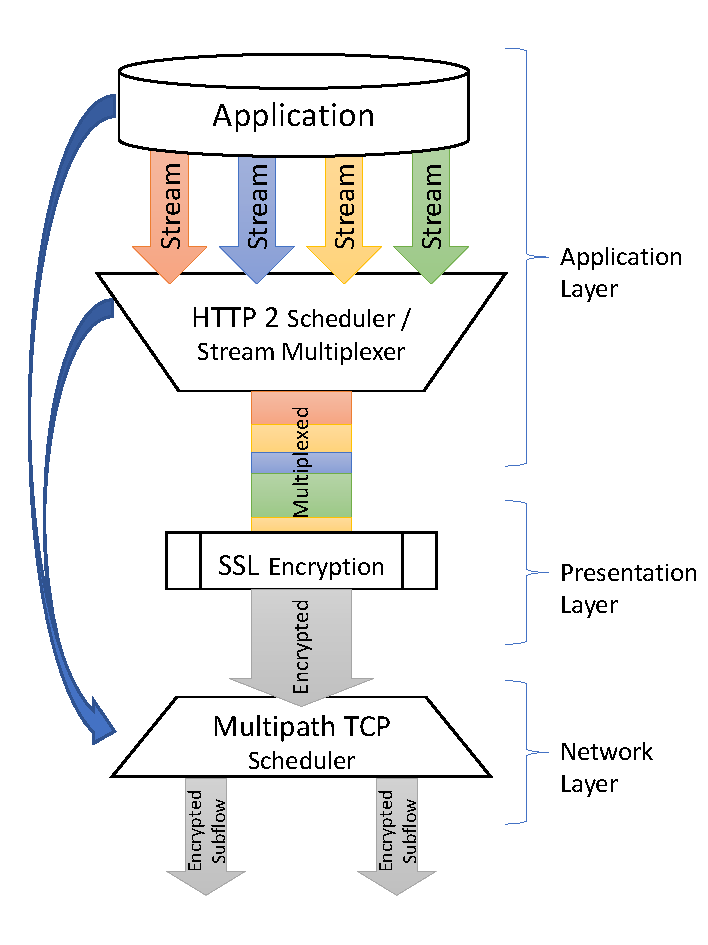
\includegraphics[width=0.45\textwidth]{mux-demux.pdf}
	\caption{Optimization across layers}
\end{wrapfigure}


% reasoning why mptcp is/will be used on devices people browse the internet with
Most smartphones and notebooks have multiple network interfaces nowadays. This has given rise to the design of various network protocols with the aim of extending bandwidth, enhancing reliability and lowering power consumption by intelligently combining interfaces. One of these is Multipath TCP  \cite{RFC6824_MPTCP}, an extension to the Transmission Control Protocol with support for combining multiple paths over multiple interfaces into a single TCP connection with higher bandwidth and reliability.


% users expect faster/instant reaction from computers/web pages/interactive services ^= do not accept (long) wait times
% web sites getting more complex
% 
% very short intro to mptcp, evtl. richtung vorteile f�r clients/webbrowsing
% ``more and more devices are mobile''
% ``almost every modern device has multiple network interfaces'' (smartphones cell+wifi, notebooks eth+wifi(+cell), desktops eth+wifi, household routers with multi uplink dsl+lte, etc)



Inherent in Multipath TCP operation is some overhead of discovering and establishing multiple paths when the connection is set up. In regular web browsing, HTTP up to version 1.1 use many short-lived TCP connections, so the overhead of multipath initialization can shatter the performance improvements of Multipath TCP, as the connection often is closed before the second path is usable. Combined with unadapted browsers, this can cause Multipath TCP to perform worse than single path TCP \cite{han2015mwebmptcp}.


% very short intro to http/2, maybe difference to http/1(.1)
% ``websites become more intricate''
The web has come a long way since the introduction of HTTP/0.9 in 1993. Many small improvements have been made in the meantime, all carefully providing backward compatibility. But web applications have become so intricate, and users so accustomed to responsive interactive services, that a clear break had to be made. Therefore, HTTP/2 \cite{RFC7540_HTTP2} has been specified. To allow easier adoption, the semantics were kept intact, while the underlying protocol was changed completely: An only seemingly simple text-based protocol was replaced with a more efficient and precisely specified binary protocol. 
The new feature most relevant to us are multiplexed streams which allow all data to be transferred over few, long-lived, thus more efficient TCP connections. The multiplexing also prevents head-of-line blocking and allows prioritizing the most time-critical resources.

% two schedulers (
% - http2 schedules frames from multiple streams into one tls/tcp connection, mostly based on http2 priority;
% - mptcp schedules tcp segments from one meta socket onto multiple real sockets
% )
% three layers

As opposed to older versions, HTTP/2 is based on long-lived TCP connections. Therefore, it can utilize the additional sub-flow capacity more often. During a single connection, different types of requests are processed, including loading a document and resources required to display it, loading auxiliary content like images below the fold, and user-initiated AJAX requests. Every type of request has different performance needs, which makes it especially interesting for cooperation-based optimization approaches.

% different scheduling approaches for mptcp are possible, many have been proposed and some are implemented in the linux kernel

% assumption: choosing best possible scheduling strategy depends on requirements of(/knowledge about/knowledge available to implementation of) higher level protocols 
% even for one given protocol, these requirements can change during a connection (e.g. web site: initial loading should be fast - user is waiting - use fastest flow(s)/use redundancy, loading of images below the fold don't need to be as fast -> conserve power/metered traffic, ajax requests might be small, but latency critical -> redundancy)
We assume that choosing the best possible Multipath TCP subflow scheduling strategy depends on information about the higher layers. In the case of HTTP/2 connections this information includes the type of the request as indicated above. For having this information available to the packet scheduler -- part of the transport layer -- there are several possible solutions, each coming with different pros and cons. 
% for some protocols, a good heuristical approach can be chosen based on transmitted bytes, time, transmission pauses, etc
For one, a heuristic approach can be chosen, which acts on metadata readily available in the transport layer, including transmission rate and pauses, elapsed time, and byte and packet counters. A positive aspect of this approach is its independency from the specific implementation of the application protocol, and that it can even work unchanged for several similar protocols. 
% for some protocols, the scheduler could look into the octet stream and decide depending on contents
% problems:
% -> breaks separation of layers - high ``dirty hack'' factor
% -> protocol decoding needs to be implemented in scheduler (os kernel!) -> proto updates need kernel updates, security problems (protocol parser is huge attack surface)
% -> impossible with encrypted protocols (not technically impossible, but would be very complicated and has performance hit)
Even more information about the state of higher level protocols can be gained by inspecting the octet stream itself. This brings with it all problems of Deep Packet Inspection, including security risks and increased code complexity \cite{Porter2005}. It is also not applicable to HTTP/2 as all browsers implement it with forced TLS encryption, therefore this approach is not considered any further.
% solution / our approach: the implementation of the higher-level protocol provides special scheduling hints to the mptcp scheduler
% pro
% - no detailed knowledge about the protocol is necessary in the scheduler
% - with a good api, the scheduler needs to know nothing about the specific application level protocol, while the app level proto implementation needs to know (almost) nothing about the transport level scheduling
% contra
% - every application which should take advantage of this approach needs to be specifically modified
% - 
The middle course we suggest is providing an API which allows the application to provide scheduling hints to the transport layer. This has the advantage of not embedding knowledge about the application layer protocol in the scheduler, thereby keeping the abstraction layers separate.


%---------------------------------------------------------------------
\section{Approach}
%---------------------------------------------------------------------

%\todob{conceptual approach}
%wie vorgehen - konzeptioneller approach
%interaction / dependency -> l�sen durch cooperation
We start by analysing the general structure of popular web sites regarding the resources on the critical path. In comparison, we look at guidelines for performance optimization in web design. 
From the gained insights, we conceive possible optimizations for existing, modified or specially crafted web pages at the transport level. The Multipath TCP implementation \cite{multipathtcp} consists of three major building blocks: path manager, packet scheduler and connection to the subflows \cite{RFC6182}. In this thesis, we pay special attention to the packet scheduler. More precisely, we concentrate on its component which spreads individual segments over subflows. These optimized schedulers are implemented in rule-based scripts which are loaded into the MPTCP implementation in the Linux kernel. To make scheduling hints like content type, priorities or dependencies available to the scheduler scripts, we modify a suitable HTTP/2-capable web server to pass on these hints as socket options. 

%auch implement. und eval approach
The next step is an evaluation of the implemented optimizations in simulated network environments. Web sites are loaded in network scenarios differing in bandwidth, round-trip time and packet loss. To study the practicality, we conduct real-world measurements for the best-performing optimizations, connecting from LTE and domestic ADSL access networks to virtual servers at a cloud provider. 



%


%---------------------------------------------------------------------
\section{Structure}
%---------------------------------------------------------------------
% where we provide an overview of the chapters

% background/rel. work
In the following chapter, we introduce the protocols on which this work is based. This is Multipath TCP on the transport layer, which is described with a focus on scheduling. On the application layer, it is the HTTP/2 protocol and its underlying concepts. A review of related publications is conducted, with a focus on Multipath TCP scheduling, coordination among software layers, cooperation between kernel and user-space components, web page optimization, and performance measurement of web pages and applications.

%approach
Chapter four starts with an analysis of typical web page structures, details our approach for passing scheduling hints from application to transport layer and presents MPTCP scheduler optimization strategies for different network scenarios. We also consider security concerns regarding the scheduling hints as a side channel to TLS encryption.

%implementation
Following our approach of integrating multiple layers, the implementation described in chapter five ranges from the transport layer up to the application layer. Optimized schedulers are realized with a scripting-enabled rule-based scheduler in the Linux kernel. After conducting a survey of web server software, we choose one to customize. This is necessary to pass information about HTTP transactions down the stack, bypassing encryption. On top of that, we implement software to evaluate web page performance.


%evaluation
To show which optimizations are worth using in which network situations, in chapter five, we evaluate the performance of the implemented schedulers in simulated and real-world networks. We conduct measurements including the resource usage, like transmitted data volume per interface, and record timestamps of all events in the browser, to calculate various page load speed metrics. Based on that data, we relate the added value for the user to potential computational overhead and bandwidth costs.


%their actual and perceived speed, utility to the user, overall and per-interface bandwidth usage, (power usage?), computational overhead, implementation difficulty, 

%conclusion
Finally, a conclusion is drawn on the accomplished improvements, which approaches were successful and which less so. The last chapter is also used to point out possible approaches for future investigations in this field.


%problem statement

% analysis of the possible ways for interaction between transport and application layer in the case of MPTCP and HTTP2

% analysis of typical web page structures

% design and implementation of MPTCP scheduler(s) for optimizing web page loading / web app usage, which get (out of band) information from presentation layer TLS, application layer HTTP2 and/or  application layer HTML, JS,... (Web Page Structure)

% evaluation of the optimizations





%=====================================================================
\chapter{Background and Related Work}
%=====================================================================

%related work
In this chapter, we go through transport, presentation and application layer, the OSI layers this work is concerned with. For each layer, we explain the relevant protocols and implementations. We will also present previous work on the optimization and measurement of web page performance.


\section{Transport Layer: Multipath TCP}


%
%http://www.ip-insider.de/anwendungen-und-konkurrenz-fuer-multipath-tcp-a-445245/
%

Two pipes are better than one - that's Multipath TCP put in a nutshell. In this case, a pipe is a distinct path between two devices, identified by the IP addresses of both peers. Combining multiple of these subflows can provide several advantages: Higher throughput can be achieved by multiplexing data over multiple subflows. The reliability of a connection can be improved by establishing backup subflows: in case a subflow stops working, the backup takes over seamlessly. \cite{Raiciu:2011:IDP:2018436.2018467} On routes with packet loss, the latency can be reduced by sending packets redundantly on multiple subflows.

This section covers the background knowledge on Multipath TCP which is required for the remaining work. We start by enumerating the current software implementations of Multipath TCP and giving some information on its current deployment. Following that, we describe the architecture of protocol and implementations. We present studies evaluating and optimizing Multipath TCP performance, and proposals and implementations of interfaces to the application layer. To finish this section, we explain the rule-based scheduler, a Multipath TCP packet scheduler, which makes its decisions based on script programs which are changeable during runtime, allowing us to evaluate different scheduling approaches faster.

%tuple of (source address, source port, destination address, destination port).





\subsection{Architecture of Multipath TCP}
%Following that, we describe the architecture of the Multipath TCP protocol and implementation. 

\textcite{Ford2008} propose that endpoint addressing and congestion control 
should be factored out of the Internet transport layer into a separate 
Endpoint Layer and Flow Layer, respectively, to address ``roadblocks to 
Internet evolution'' caused by the fact that middleboxes such as ``firewalls 
and NATs must understand transport headers''.
In RFC 6182, \textcite{RFC6182} explain that the architectural design of 
Multipath TCP is based on this idea, decomposing the transport layer 
functions into application-oriented and network-oriented parts. They describe 
``the subflow TCP
component, which provides network compatibility by appearing and
behaving as a TCP flow in the network [as] an instantiation of the
`network-oriented' Flow+Endpoint layer''. 
It is acknowledged that at this layer end-to-end service can't be expected 
as ``Middleboxes routinely interpose on the transport layer''.
This compatibility is considered important to allow deploying it in the 
current Internet landscape.

The ``\thinspace`application-oriented' Semantic layer'' of Multipath TCP provides ``
application compatibility through the preservation of TCP-like semantics of 
global ordering of application data and reliability''. Combined with a 
backward compatible API this allows ``that existing applications can use the 
newer transport merely by upgrading the operating systems of the end hosts''.

According to \textcite{RFC6182} a Multipath TCP implementation must provide 
the following features: (a) path management, to find paths and establish new 
subflows between the peers; (b) packet scheduling, to split the octet stream 
into segments and decide on which subflow(s) to send each of them, and to 
reassemble them upon receiving; (c) a subflow interface, to transmit packets 
over a single path, in a way compatible with TCP; (d) shared congestion 
control for all subflows of the same connection, to ensure sharing 
bandwidth fairly at bottlenecks.  

In figure \ref{fig:mptcp-arch}, we illustrate how data flows through the 
Multipath TCP transport layer components: the application produces a stream 
of data, the packet scheduler breaks it into segments and distributes them 
across the subflow interfaces. They, in turn, add per-subflow sequence 
numbers and transmit the segments over the network layer. At the remote peer, 
segments flow in the opposite direction, while getting reordered and finally 
reassembled to an application data stream by the packet scheduler.

\begin{figure}
	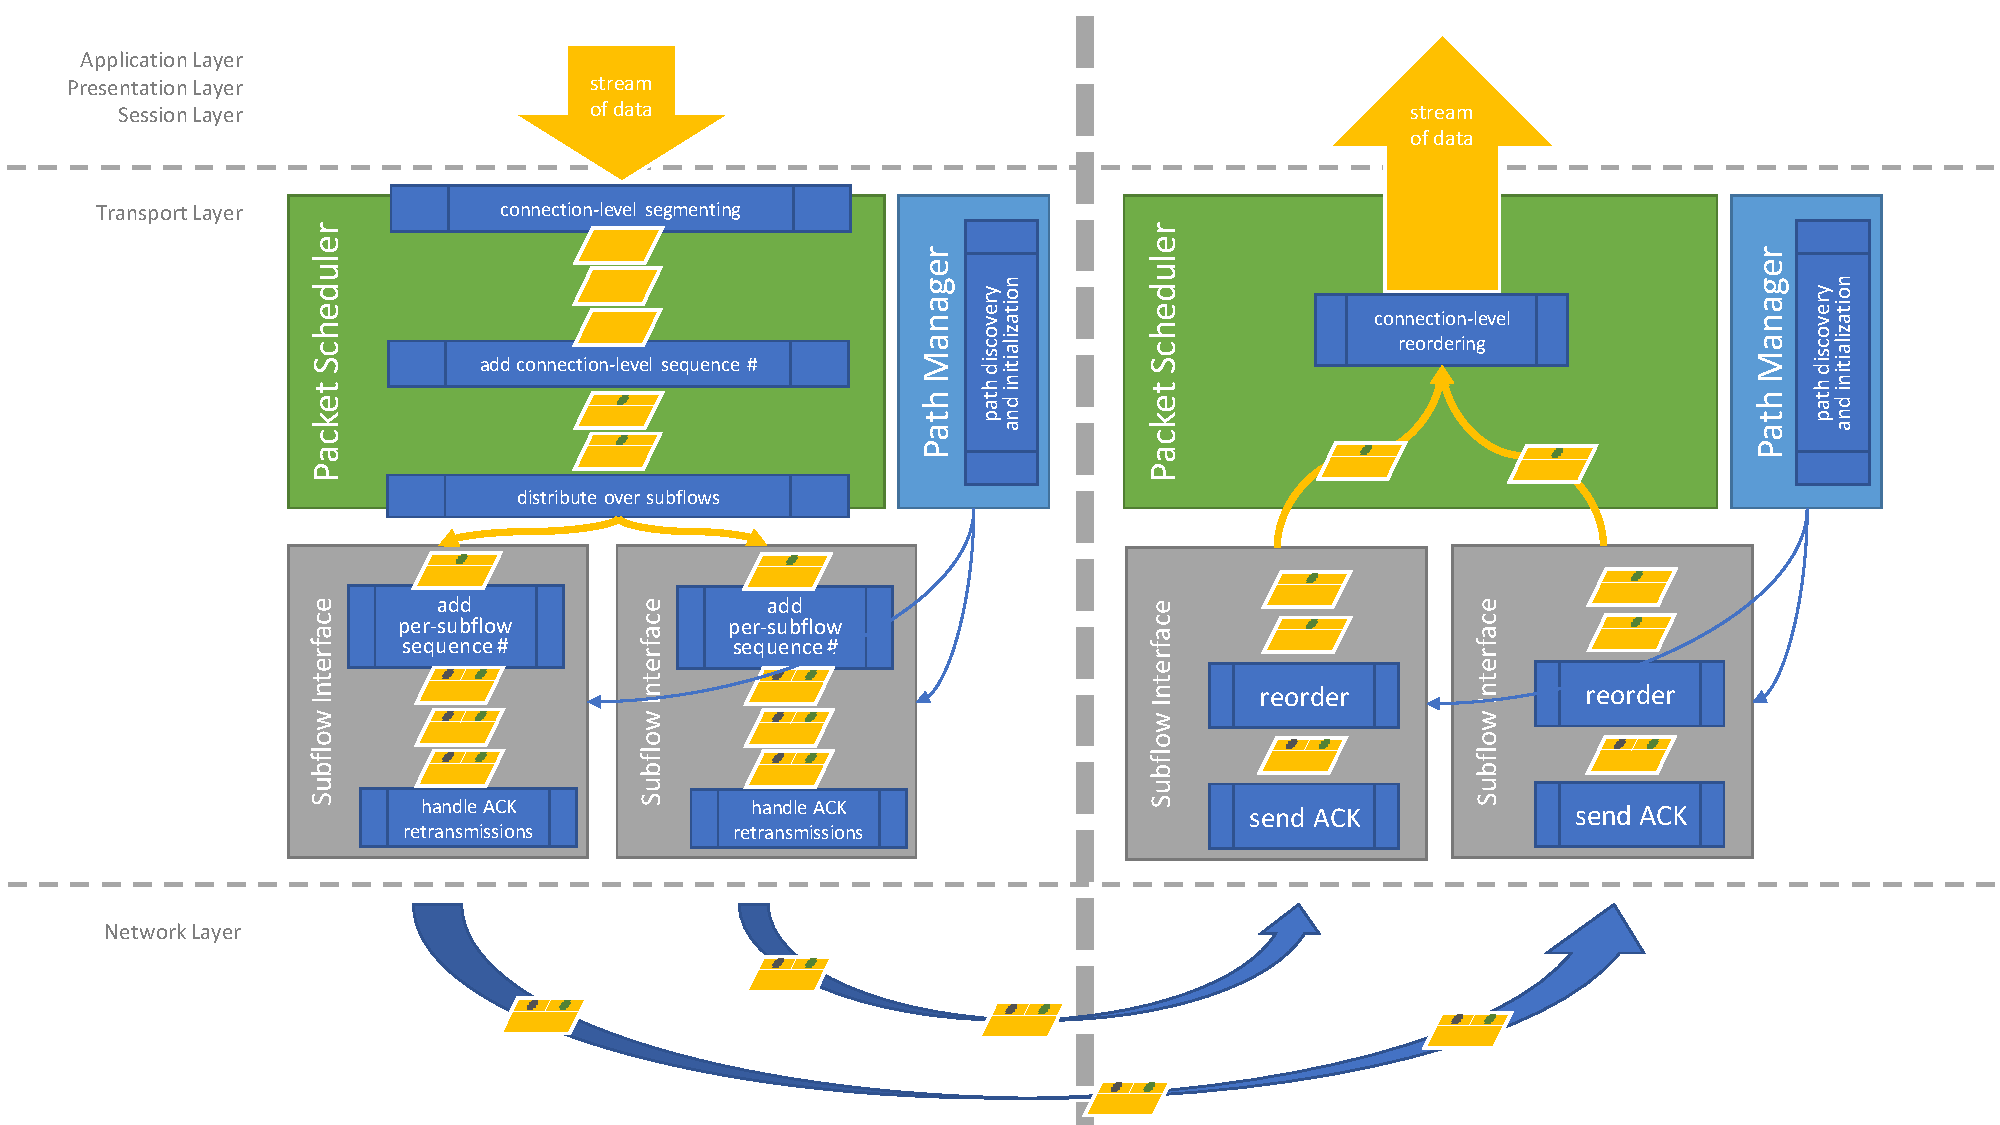
\includegraphics[width=1\textwidth]{mptcp-functional-decomposition.pdf}
	\caption{Interaction of the functional building blocks of Multipath TCP as described in \cite{RFC6182}}
	\label{fig:mptcp-arch}
\end{figure}

%\subsubsection{Path Management}



%\subsubsection{Packet Scheduling}




%\subsubsection{TCP Subflows}


%\todo{xxx}



\subsection{Multipath TCP on the Wire}
Multipath TCP subflows look and behave on the wire exactly like regular TCP 
flows, except the segments contain some additional TCP options as described 
in RFC 6824 \cite{RFC6824_MPTCP}.

When a new Multipath TCP connection is set up, the \textbf{MP\_CAPABLE} 
option is included in the SYN segment. From these options, the server learns 
that the new client supports MPTCP. In the responding SYN-ACK and ACK 
segments, the MP\_CAPABLE option is included as well, serving as a handshake, 
in which authentication keys are exchanged. These keys are later used in the 
process of adding more subflows to the connection.

New subflows are initiated by establishing what looks like a regular TCP 
connection to the network, but contains the \textbf{MP\_JOIN} option in the 
three-way handshake segments. The contents of this option depend on the 
stage of the handshake. The initiator sends an identifying token, which is 
based on the authentication keys.  In the first two segments, random numbers 
(nonces) are exchanged. To authenticate each other, the peers exchange HMACs 
of the concatenated nonces keyed on the concatenated authentication keys in 
the second and third segment.

During the regular data transmission, the \textbf{DSS} option (Data Sequence 
Signal) is added to every segment. It contains sequence numbers and 
acknowledgements, which work very similar to their TCP counterparts. They are 
necessary to ensure ordered data transfer across subflows, and to retransmit 
segments in case of collapse of a subflow.


\subsection{Implementations and Deployment}
%We start by enumerating the current software implementations of Multipath TCP and giving some information on its current deployment.

%reference(?) implementation in linux kernel
The current reference implementation\footnote{\url{http://multipath-tcp.org/}} is based on the Linux kernel and was developed by \textcite{multipathtcp} at the Universit� Catholique de Louvain. A similar patch for the FreeBSD kernel has been developed at Swinburne University\footnote{\url{http://caia.swin.edu.au/newtcp/mptcp/}}.
%https://support.apple.com/en-us/HT201373
The first implementation of Multipath TCP was written as a user-space proxy\footnote{\url{https://open-innovation.alcatel-lucent.com/projects/mptcp-proxy}} by Hampel at Bell Labs, and is no longer maintained.  
%other implementations
The most widely deployed implementation is found in Apple's XNU kernel\footnote{\url{https://opensource.apple.com/source/xnu/xnu-2422.1.72/bsd/netinet/mptcp.c.auto.html}} \cite{Hesmans2016}, used in the macOS and iOS operating systems. It is used mainly for the Siri personal assistant software, which keeps a backup connection over cellular network in case the Wi-Fi connection breaks down \footnote{\url{https://support.apple.com/en-us/HT201373}}. 
All aforementioned implementations are open source. There is also one known closed-source implementation by Citrix Networks in their load balancer firmware \cite{Eardley2013}.

% multiple network interfaces
\begin{wraptable}{r}{9cm}%
\centering
		\begin{tabular}{p{3.5cm}p{5cm}} \toprule
		Device Type    & Network Interfaces \\ \midrule
		Smartphones & Wi-Fi and cellular \\
		Notebooks & Wi-Fi, often Ethernet, sometimes cellular \\
		Desktops & Ethernet and/or Wi-Fi \\
		Servers & Ethernet (multiple) \\
		Household routers with multiple uplinks & DSL and cellular (LTE) \\ \bottomrule
		\end{tabular}
		\caption{Typical network interfaces of common device types}
		\label{table:typical-netifs}
\end{wraptable}

Korean Telecom announced a deployment on their cellular network, including the
Multipath TCP implementation in the Linux kernel of their Android phones. 
At carrier level, they provide a SOCKS proxy server, over which traffic is sent
by the Android operating system, both using Multipath TCP.
This allows combining Wi-Fi and cellular connectivity over existing infrastructure,
reaching download speeds of over 800 Mbps \cite{Bonaventure2016Deploy}.
Another deployment scenario are ``hybrid access 
networks'', where customers� networks are connected to multiple DSL links, combined 
using Multipath TCP, to achieve higher bandwidth \cite{DeConinck2016}.
In general, Multipath TCP can be deployed in scenarios where at least one peer 
has multiple interfaces. This is the case for an increasing number of device 
classes, as listed in Table \ref{table:typical-netifs}. In this work, we will 
concentrate on consumer devices with Wi-Fi and cellular interfaces.



\subsection{Socket API}
%We present [...] proposals and implementations of interfaces to the application layer.

%application api's
The only way to control the current Linux implementation from user-space was by setting \code{sysctl} parameters, which are generally valid for the entire operating system. They allow the system administrator to enable or disable Multipath TCP for all applications, and to change several high-level parameters globally. If Multipath TCP is enabled, it is used for all TCP connections and is transparent to the application. Recently, the socket option \code{MPTCP_ENABLED} was introduced, which allows switching it on or off per socket. Still, application developers don't have any fine-grained control over the Multipath TCP behaviour.

In contrast, the Apple implementation takes a very different approach by providing a new socket-based API. One the positive side, this gives Multipath TCP aware applications full control over Multipath TCP connections, setting up, enumerating and tearing down subflows. New \code{connectx} and \code{disconnectx} system calls are introduced for that reason. However, this makes it incompatible to existing applications, requiring developers to make modifications to take advantage of the new protocol.

To allow similar fine-grained control, while keeping the compatibility with unadapted applications, several APIs have been proposed. 
%RFC 6897
\textcite{Scharf2013} present in RFC 6897 a ``Basic API for MPTCP-Aware Applications'', enabling applications to restrict the interfaces to use for establishing paths and to query the subflows and their addresses. 
They also recommend that socket options on a Multipath TCP meta-socket should be, if possible, passed through to all subflow sockets.
%Hesmans 2016 - An enhanced socket API for Multipath TCP



\subsection{Performance Evaluations} \label{relwork-mptcp-performance}
%We present studies evaluating and optimizing Multipath TCP performance, [...]

%\todo{We present studies evaluating and optimizing Multipath TCP performance, [...]}

%Experimental evaluation of multipath TCP schedulers
\textcite{Paasch2014} propose a modular Multipath TCP scheduler framework in 
the Linux kernel and use this framework to evaluate schedulers in a Mininet 
simulation and in a real-world testbed. 
Schedulers compared are a round-robin (RR) scheduler, and several variations 
of a lowest-RTT-first (LowRTT) scheduler. They find that for application 
limited flows, ``the RR scheduler is particularly bad in terms of application 
delay'', but for bulk transfers, it performs like LowRTT. 
For all schedulers alike, once ``all congestion windows are filled, the 
scheduling becomes ack-clocked'', meaning that packets are always scheduled 
into the next subflow where congestion window space gets available.

They also highlight that bad schedulers can trigger head-of-line blocking: 
paths with different delays resulting in out-of-order packet arrival, forcing 
``the packets that are scheduled on the low-delay subflow [...] to `wait' for 
the high-delay subflow's packets to arrive in the out-of-order queue of the 
receiver'' to fulfil Multipath TCP's in-order delivery guarantees. 
Therefore, ``Multipath scheduling should ideally be done in a way that the 
data is received in-order.''

%Impact of Path Characteristics and Scheduling Policies on MPTCP Performance
\textcite{Arzani2014} compare Multipath TCP schedulers that only decide based 
on the congestion window of subflows to schedulers that are aware of the 
round-trip time of subflows. They found that only if the RTTs of subflows are 
substantially different, the RTT-aware scheduler performs better.
%Remp TCP: Low latency multipath TCP
\textcite{Frommgen2016a} propose a Multipath TCP scheduling algorithm which 
sends data redundantly over multiple subflows, to achieve the lowest possible 
latency at the cost of higher bandwidth usage. They evaluate it for multipath 
connections over Wi-Fi and LTE, finding that it ``more than halved the average 
round-trip time''.

Several works evaluate the influence of congestion control on Multipath TCP performance. \textcite{Raiciu:2011:IDP:2018436.2018467} compare Multipath TCP's coupled congestion control algorithm to uncoupled and equally-weighted TCP (EWTCP), finding that the former is more aggressive, gaining unfair advantage over single path TCP at bottlenecks, while EWTCP, on less loaded paths, ``misses sending opportunities and gets slightly lower throughput''.
In \textcite{Wischik2011}, ``fairness goals and RTT compensation'' are tested on devices with multiple wireless interfaces with different characteristics, as are Wi-Fi with ``much higher throughput and short RTTs, but [...] quite high loss rates'' and 3G which they ``found [...] to be overbuffered
leading to RTTs of well over a second''.
For single-flow tests, they found that ``the MPTCP user gets bandwidth roughly equal to the sum
of the bandwidths of the access links''.
They show that Multipath TCP shares bandwidth fairly with single-path TCP flows, being ``approximately as good as the better of the single-path competing flows''.

\textcite{Chen2013} evaluate the download times for files of different size 
using Multipath TCP over Wi-Fi and cellular connections to using only one of 
those interfaces alone. They found ``that MPTCP is robust in achieving 
performance at least close to the best single-path performance, across a wide 
range of network environments. For large transfers, performance is better 
than the best single path, except in cases with poor cellular networks''. 
When downloading small files, they found that Multipath TCP provides benefits 
as it ``leverages [multiple] slow-start phases simultaneously to fetch the 
one file''.
\cite{DeConinck2016} traced Multipath TCP on smartphones with real apps and 
users by relaying all traffic over a MPTCP-enabled proxy server and analyse
results regarding subflow setup and usage, network RTTs, connection handovers 
and packet reordering and reinjection. Findings include that there is some 
overhead as many subflows are established but never used, and that long 
connections benefit from seamless handovers.


They also provide useful data on performance characteristics of Wi-Fi and 
cellular networks. Mobile 4G connections have specified maximum data rates of 
100 Mbps. They observed that packet ``loss rates over 3G/4G networks are 
generally lower than 0.1\%, while those of WiFi vary from 1\% to 3\%''. The 
low loss rates are bought at the price of higher RTTs, as cellular operators 
use local retransmission mechanisms to avoid TCP identifying the packet as 
lost and regarding the link as congested. RTTs are reported as 30 ms on 
average for Wi-Fi connections, and at least 60 ms for cellular connections.
 


\subsection{Rule-Based Scheduler}
The rule-based scheduler by \textcite{RBS} is a programmable Multipath TCP scheduler. The scheduler programs are written in the RBS scripting language. They are just-in-time compiled to byte code and executed by a virtual machine in the scheduler for every scheduling decision. They can be loaded dynamically without having to recompile the Linux kernel and reboot the system. This allows us to change algorithms and evaluate different scheduling approaches quickly.


\paragraph{Scheduler Scripts}

In the later chapters, we show several scheduler scripts written in the RBS language. To allow the reader to follow these scripts, we give an introduction to the core objects used in the scripts.
The syntax of RBS is similar to C, separating statements with the semicolon and using braces for blocks. A visible difference is that keywords are written in upper-case. The \textbf{control flow elements} available are if statements in the form \texttt{IF (condition) \{ ... \} ELSE \{ ... \}}; and a loop to iterate over all elements in a list as \texttt{FOREACH (VAR item IN list) \{ ... \}}. The execution of a script can be stopped at any point with the \code{RETURN} statement. 

%\paragraph{Variables and Registers}

\textbf{Variables} are always immutable and can be declared and assigned with \code{VAR myVariable = ...}. They keep their value only during the current script execution. To store state across calls to the scheduler, the \textbf{registers} R1 to R6 can be used. They are always of type integer, therefore it's not possible to store objects or lists of objects permanently. To assign a register, the SET function is called like this: \code{SET(R1, 42)}.


%\paragraph{Queues, Lists and Objects}
The \code{Q} and \code{RQ} variables provide access to \textbf{packet list} objects, 
containing the sending queue and the retransmission queue, respectively. As 
long as any of these queues contains packets, the script is run in an 
implicit loop. Therefore, no loop over available packets is necessary in the 
script. As queues, they provide access to the top element through the 
\code{TOP} attribute and the \code{POP()} method. The \code{QU} list contains 
all unacknowledged packets. Table \ref{tab:skb-attrs} lists the attributes and 
methods providing information about a packet.
The \code{SUBFLOWS} variable contains the list of all \textbf{subflows}. In table 
\ref{tab:subflow-attrs} the attributes of a subflow object are explained.

\textbf{Lists} provide several methods which facilitate a functional programming approach by using 
an anonymous function as a parameter to filter, sort or aggregate the list: 
\code{FILTER} returns a list containing all elements for which the expression 
evaluates to TRUE; \code{MAX} and \code{MIN} return the element for which the 
expression produces the greatest or smallest value, respectively; and 
\code{SUM} calculates the sum of the expression evaluated on every list element.
They also all have \code{COUNT} and \code{EMPTY} attributes available. 

% subflow attributes
\begin{table}[h]
	\begin{tabularx}{\linewidth}{ l X } \toprule
	Attribute & Description \\ \midrule
	\code{ID}								& Numeric identifier of the subflow. Unique per MPTCP connection. \\
	\code{RTT} 							& Calculated round-trip time on this subflow in milliseconds. \\
	\code{LOST_SKBS} 				& Number of packets which were lost on this subflow. \\
	\code{SKBS_IN_FLIGHT} & Number of packets which were sent out on this subflow but not yet acknowledged or retransmitted. \\
	\code{CWND} 						& Congestion window. Number of packets which are allowed to be in flight on this subflow at the same time. \\
	\code{IS_BACKUP} 			& Boolean flag, \code{TRUE} if subflow is marked as a backup subflow by the user or operating system. \\
	\bottomrule
	\end{tabularx}
	\caption{Subflow details as seen from the RBS script}
	\label{tab:subflow-attrs}
\end{table}

% buffer attributes
\begin{table}[h]
	\begin{tabularx}{\linewidth}{ l X } \toprule
	Attribute & Description \\ \midrule
	\code{USER}								& Application-defined parameter (set via \code{setsockopt}). \\
	
	\texttt{SENT\_ON(\textit{<subflow>})} 							& Boolean flag, \code{TRUE} if the packet has been sent on the given subflow. \\
	\code{SENT_ON_ALL} 				& Boolean flag, \code{TRUE} if the packet has been sent all subflows. \\
	
	\bottomrule
	\end{tabularx}
	\caption{Packet properties}
	\label{tab:skb-attrs}
\end{table}



\paragraph{Scheduling Packets}
To actually schedule a packet onto a subflow, the PUSH method of a subflow is 
called. Listing \ref{lst:schedule-a-packet} shows the idioms for scheduling a 
packet on one or multiple subflows. To make sure that no packet is 
inadvertently dropped, the \code{<packet list>.POP()} method can only be 
called inside a PUSH or DROP statement.

\begin{lstlisting}[style=RBS,label=lst:schedule-a-packet,caption={Schedule a packet from Q}]
/* single subflow in ``sbf'' */
sbf.PUSH(Q.POP());

/* list of subflows in ``sbfs'' */
IF (!sbfs.EMPTY) {
	FOREACH(VAR sbf IN sbfs) {
		sbf.PUSH(Q.TOP);
	}
	DROP(Q.POP());
}
\end{lstlisting}


\paragraph{Socket Kernel Buffers} \label{skb-annotate}

%something about the annotated socket buffers a.k.a. USER field
As a packet goes through the Linux network stack, it is stored in a socket 
kernel buffer (SKB)\footnote{for more information, see 
\url{http://vger.kernel.org/~davem/skb.html}}. When an application sends 
data over a TCP connection, it can call the \code{write} method, which 
will either append the data to an existing SKB, or store it in a newly 
created one. 
The SKB contains the data itself, pointers to the socket, network device 
and various other structures, and a data area which can be used by the 
transport protocol. For the RBS, this data area is extended to store the 
\code{USER} field, a byte with user-defined meaning, which can be set by the 
application and read by the scheduler script. The application can use the 
\code{setsockopt} call to set the field value for the data which is sent with 
the following \code{write}s.






\section{Presentation Layer: TLS} \label{tls-background}

We need to consider Transport Layer Security (TLS) in this work as all browser 
implementations of the HTTP/2 protocol enforce the usage of encryption by 
TLS\footnote{\url{http://caniuse.com/\#search=http2}}.
Put another way, to use HTTP/2, we need to use HTTPS. 
On the other hand, TLS is relevant anyway for evaluations of web traffic, as it 
is used by a growing portion of web sites. \textcite{naylor2014cost} states 
that ``[i]n September 2014, 44.3\% of web connections already use HTTPS'', and 
according to Mozilla Telemetry\footnote{\url{https://telemetry.mozilla.org/new-pipeline/dist.html\#!cumulative=0&end_date=2017-03-24&keys=__none__!__none__!__none__&max_channel_version=release\%252F52&measure=HTTP_PAGELOAD_IS_SSL&min_channel_version=null&processType=*&product=Firefox!Fennec&sanitize=1&sort_keys=submissions&start_date=2017-03-02&table=0&trim=1&use_submission_date=0}}, 
55\% of HTTP page loads were over SSL in March 2017. %Therefore, we researched the performance impacts of TLS usage. 
% why we need to consider ssl
% - x% of connections use ssl today

%``The growth of HTTPS adoption is striking, with the HTTPS ?ow share more than doubling in two years.''
%``the �S� is here to stay''


The intermediate layer of TLS complicates the collaboration of application and 
transport layer. We can't look at the HTTP/2 traffic from our Multipath TCP 
scheduler, as it is always encrypted. We can't pass metadata based on byte 
ranges or sequence numbers, either, because TLS chops the data into records, 
adding headers in front and padding at the end of each record.

What makes things easier, is the fact that the most common TLS library 
``OpenSSL will build a record from each call to SSL\_write'' \cite{Langley2010}, 
which means there is no internal buffering, which otherwise would have further confused the 
relationship between plain and encrypted data. Therefore, it is possible to
use the mechanism described in Section \ref{skb-annotate} to pass metadata
to schedulers, and to view \code{SSL_write} as equivalent to \code{write}.
%  therefore collab. via socket option no problem -> correctness

%Closely related to this is the fact that choosing the right size for TLS record 
%can have considerable impact on performance. 



%``the TLS standard provides a fast negotiation mechanism, which reduces the TCP+TLS handshake to 2 RTTs'' (session id)




\section{Application Layer: HTTP/2 and HTML}

The HyperText Transfer Protocol (HTTP) is the protocol which is used by web 
browsers to load web sites from web servers. But since its inception in 1993, 
web sites have changed a lot, which caused the need for improvements in HTTP. 
For example, modern web sites often consist of hundreds of individual files 
and have interactive components. With classic HTTP/1.0, a new TCP connection 
is established for every file download, which needs three round trips. If 
encryption is used, an individual TLS handshake is performed as well, which 
needs another four round trips. To improve the situation, connection keep-alive
and request pipelining was introduced with HTTP/1.1, allowing to use 
the same connection for multiple downloads. However, the responses have to be 
sent by the server in the same order as the requests were made, leading to 
the problem of head-of-line blocking when the earlier responses take longer 
to compute at the server.
Another problem is the verbosity of the text-based HTTP/1. The meta data 
(HTTP header) is transmitted as human-readable text, which makes debugging 
easier, but uses more bandwidth and is more complex to parse. Compressing the 
headers with algorithms like gzip has caused security problems and was 
therefore not pursued.



As we have seen, there are many issues with classic HTTP, and many small 
improvements have been made, all carefully providing backward compatibility. 
But web applications have become so intricate, and users so accustomed to 
responsive interactive services, that a clear break had to be made. 
Therefore, HTTP/2 \cite{RFC7540_HTTP2} has been specified. To allow easier 
adaption, the semantics were kept intact, while the underlying protocol was 
changed completely: the only seemingly simple text-based protocol was 
replaced with a more efficient, precisely specified binary protocol. 
The new feature most relevant to us are multiplexed streams which allow all 
data to be transferred over fewer, long-lived, thus more efficient TCP 
connections. The multiplexing also avoids head-of-line blocking and allows 
prioritizing the most time-critical resources.


%``HTTP/2 is a binary, rather than text, protocol, making it more compact and efficient
%It uses a single, multiplexed connection per domain, rather than multiple connections carrying one file each
%Headers are compressed with the purpose-built HPACK protocol (rather than gzip, as in SPDY)
%HTTP/2 has a complex prioritization scheme to help browsers request the most-needed files first, which is fully supported in NGINX (SPDY had a simpler scheme)''
%https://www.nginx.com/blog/7-tips-for-faster-http2-performance/

\subsection{Frames, Streams and Priorities} \label{http2-frame-types}

%\todo{wie sehen frames aus und welche typen gibt es -> zusammenfassen aus http/2 spec}

On the wire, HTTP/2 is a framed protocol. A connection is started with a 
connection preface sent by client, which is a fixed sequence of 24 bytes. 
After that, all data is exchanged in frames. The first frame the server sends 
is always of type SETTINGS. 
A frame consists of a 9-byte header, followed by data whose length is 
specified in the header. Besides the header contains the frame type, 
type-specific flags, a reserved bit, and a stream identifier.

In the specification \cite{RFC7540_HTTP2}, ten frame types are defined: the 
DATA frame, which is used to transmit request and response payloads, as 
well as optional padding; the HEADERS and CONTINUATION frame types, carrying 
the HTTP headers of a request or response; the PRIORITY frame the browser can 
use to specify the priority of a stream; the RST\_STREAM frame which can be 
used to immediately close a stream; the SETTINGS frame which is used as a 
handshake at connection setup, and can also be sent later to change various 
connection settings; the PUSH\_PROMISE sent by the server to inform the 
client of a server-push stream; the PING frame as a heartbeat of idle 
connections; the GOAWAY frame to close a stream or the whole connection in 
case of errors; and WINDOW\_UPDATE for HTTP/2's internal flow control 
mechanism.

\clearpage

\begin{wrapfigure}{r}{0.57\textwidth}
\centering
	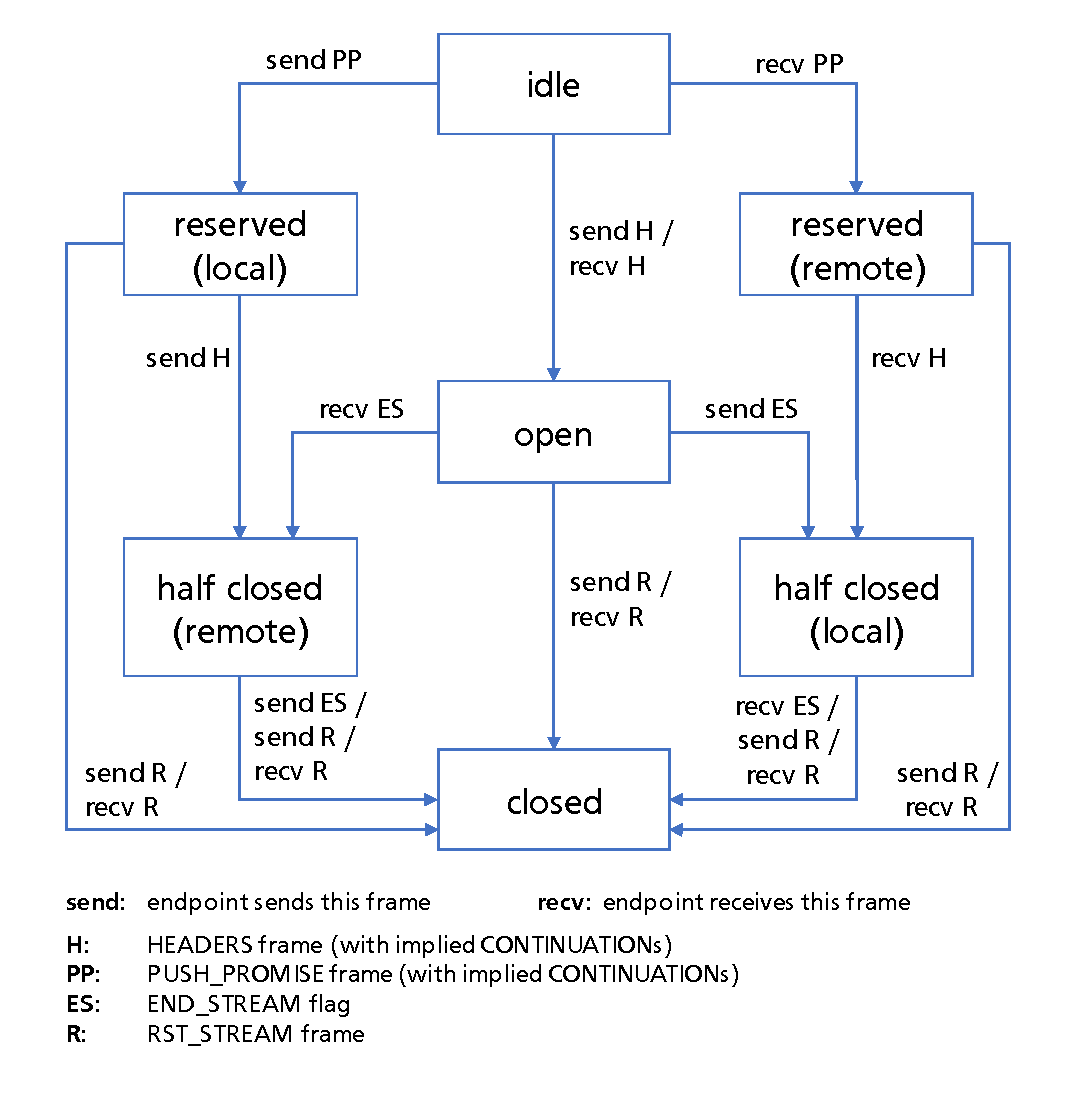
\includegraphics[width=0.57\textwidth]{http2-state-machine.pdf}
	\caption{HTTP/2 Stream State Machine \cite{RFC7540_HTTP2}}
	\label{http2-state-machine}
\end{wrapfigure}

HTTP/2 defines a complex state machine of stream states visualized in 
Figure \ref{http2-state-machine}, similar to the TCP state machine. No
three-way handshake is necessary as the identity of the 
other peer is guaranteed by the underlying protocols.
The HEADERS frame has a dual role: it is also used as one of two ways to open a new stream 
when sent with a new stream identifier. The other way is a PUSH\_PROMISE sent by the server,
which initializes a stream in the ``reserved'' state, in which the client either waits for the
promised data, or rejects it with a RST\_STREAM. By setting the END\_STREAM flag on
a packet, an endpoint can notify its peer that it will send no more data on
this stream, sending the stream in the ``half-closed'' state. Once the peer
answers with an END\_STREAM, the stream is considered ``closed''.

The priority of a stream can be included in the HEADERS frame, and changed 
at any time by sending a PRIORITY frame. It is expressed as a recursive
dependency on other streams, combined with a weighting factor to give the
priority of stream relative to its siblings depending on the same parent stream.





\subsection{Application Layer Protocol Negotiation}

% newer openssl version (apls support)
HTTP/2 can be used over the same TCP port as older versions, so browser and 
server need to negotiate the version. When using HTTP/2 over TLS, as is the 
only way to use in current browsers, this negotiation is done during the TLS 
handshake. Two different protocol extensions to TLS have been defined for 
this purpose. The older one, Next Protocol Negotiation (NPN) was defined in 
2012 for the SPDY protocol, a precursor of HTTP/2. It is replaced by the more
recent Application Layer Protocol Negotiation, defined as an official
TLS extension in 2014 \cite{RFC7301}. The two 
protocols are very similar; the only difference is that with NPN the negotiation
was encrypted, while APLN adapted to the common TLS practice of conducting
negotiations in the clear.
In any case, we need to use APLN, as that is what modern versions of Chrome 
and Firefox require, while OpenSSL version 1.0.1, which is available in Debian 
and Ubuntu repositories only supports NPN. Therefore, we need to build a more 
recent OpenSSL version from source if using these distributions.



\section{Web Performance}

\textcite{klotski2015} argue that web page complexity grows faster than network performance, making ``protocol-, network-, and browser-level optimizations [...] largely ineffective''. As a contradictory trend, they cite ``studies [that] suggest most users have a tolerance of at most 5 seconds'' waiting time.
They propose the ``KLOTSKI'' system to reprioritize the web resources according to their utility to the user via a proxy server. A back-end service extracts page's dependency structure and resource load times, creating a page fingerprint. The web proxy prioritizes the resources using the user's preferences and the page fingerprint, heuristically selecting the subset of the page's resources with highest utility which can be loaded in the configured user tolerance time.
They decided not to ``block or filter any content, so as to not risk rendering websites unusable''.







\textcite{han2015mwebmptcp} conducted a ``measurement study of mobile web performance over multipath TCP'', focusing on interactions of application (web) and transport layer.
Inherent in Multipath TCP operation is some overhead of discovering and establishing multiple paths, especially during connection setup. Older versions of HTTP use many short-lived TCP connections, so the overhead of multipath initialization can shatter the performance improvements of Multipath TCP. Combined with unmatched expectations of the browser, there are situations where Multipath TCP can hurt the HTTP/1.1 performance compared with single path TCP. 
HTTP/2 is better suited to use with Multipath TCP, as many small requests are coalesced into one long-running TCP connection.  This causes the overhead of establishing subflows to get less significant, the additional sub-flow capacity is utilized better as less time is spent in TCP slow start mode, so it can benefit from combined throughput of multiple paths. The same benefits can be enjoyed for long-running HTTP/1.1 connections, e.g. when downloading large files. 
They also introduce the \code{tcpdump-mpw} tool, which is used to analyse the cross-layer effects of HTTP/SPDY transactions over Multipath TCP, providing, among other things, the amount of data transferred per transaction per subflow.





%	1. PageLoadTime (Zeit bis Load Event)
%	2. Zeit bis DOMContentLoaded Event
%	3. First Paint / First Contentful Paint / First Meaningful Paint
%	> First Meaningful Paint is essentially the paint after which the biggest above-the-fold layout change has happened, and web fonts have loaded. See the spec to learn more: First Meaningful Paint: A Layout-Based Aproach.
%	https://developers.google.com/web/tools/lighthouse/audits/first-meaningful-paint
%	``Time to First Meaningful Paint: A layout-based approach''
%	https://docs.google.com/document/d/1BR94tJdZLsin5poeet0XoTW60M0SjvOJQttKT-JK8HI/view#heading=h.tdqghbi9ia5d

%1 und 2 sind �ber chrome remote debugging api leicht erh�ltlich (Page.loadEventFired)
%3 ist im Devtools Timeline view sichtbar, muss also auch �ber das remote debugging api verf�gbar sein (Devtools verwenden selber auch das rda)

%Chrome Debugging - Tracing
%https://chromedevtools.github.io/debugger-protocol-viewer/tot/Tracing/
%https://docs.google.com/document/d/1CvAClvFfyA5R-PhYUmn5OOQtYMH4h6I0nSsKchNAySU/edit



%\subsection{Categorizing web page components}

%Automatische Einstufung von Seitenbestandteilen (HTTP Requests) in Relevanz / User Utility
%-> nicht Thema der Arbeit, aber evtl. relevant f�r praktische Umsetzung

%Automatisches Aufbauen von Dependency Graphs



%HTTP/1.1 mostly benefits from Multipath TCP for larger file downloads because the TCP connections are often closed after one download, whereas the overhead of establishing auxilliary paths is not worthwile for downloading only one small file. In some studies it has been shown that the HTTP/1.1 performance is worse with MPTCP that with single path TCP on the same connection. Especially the common HTTP/1.1 optimization practice of sharding (spreading files among many different origins).
 
\section{Cooperation of Protocol Layers}

% research: what kinds of information that one layer has available, could provide an advantage to an other layer

\textcite{Raisinghani_2004} elaborate the various ways of providing feedback 
across protocol layers. They say that the ``application layer can communicate 
to other layers the application's QoS needs, i.e. the delay tolerance, 
acceptable delay variation, required throughput and acceptable packet loss 
rate''. In detail, they list devices with multiple network interfaces as
a potential application field for cross-layer feedback, because ``a wireless 
LAN interface may provide lesser delays and higher throughput as compared to a 
GPRS interface on the same device. Depending on the application or user needs,
the network layer could select an appropriate network interface.'' 
With Multipath TCP, we can do this, at the transport layer, even in a more 
fine-grained way, changing the priorities of subflows or sending data 
redundantly over multiple subflows.


\textcite{nowlan2012unorderedtcp} argue that many modern applications use TCP 
as a substrate rather than an abstraction, converting ``TCP's in-order 
semantics from a convenience blessing to a performance curse''.
Therefore, they propose a wire-compatible extension to the
TCP and TLS protocols, allowing out-of-order delivery for latency-critical 
applications while remaining compatible with TCP-only middleboxes. 





%=====================================================================
\chapter{Approach}
%=====================================================================


	
%Annahmen:
We will describe a few assumptions made for the implementation and all optimizations.
%TCP-Verbindung wird immer vom Browser aufgebaut
First, we always look at a MPTCP connection which is established by the web browser and accepted by the web server. This is always the case for HTTP connections.
%Nur der Client/Browser hat mehrere Interfaces / sendet MP JOIN Anfragen -> path-manager erstmal nicht relevant
Only the client has two interfaces with different network addresses. After the connection is set up, it directly opens the second subflow by connecting to the server from the secondary interface with a \code{MP_JOIN} option in the \code{SYN}. The server has only one (visible) interface and accepts the second subflow. Therefore, we won't discuss different MPTCP path management algorithms.
%Client hat zwei Interfaces (Wi-Fi und 3G)
The client's interfaces are either Wi-Fi and 3G/LTE, as found on smartphones, or Ethernet and Wi-Fi, which is common for notebooks.
%Kontrollierbare Aspekte: 
%	- Scheduler
%	- TCP Flow Control/Congestion Control


\section{Metrics for Web Performance } \label{metrics-web-perf}



When evaluating the performance of web page loads, there are several metrics 
to look at. We use three timing metrics, which are available in the Google 
Chrome web browser's developer tools.

%Parameters/Properties/Values: (in order of usual occurence)
% ...stimmt nicht,domcontentloaded und firstmeaningfulpaint k�nnen in beliebiger abfolge auftreten, je nach dem wie die webseite angelegt/optimiert ist


% DOMContentLoaded
The \textit{DOMContentLoaded} event is fired after the main HTML document has 
been fully received and parsed by the browser \cite[section 12.2.6]{HtmlStandard}. 
As the parsing is blocked by synchronous JavaScript\footnote{Modern browsers 
use ``speculative parsing'', where parsing continues while waiting for the 
synchronous JavaScript to be loaded and run. Still, the browser can only fire 
\textit{DOMContentLoaded} after running all synchronous scripts, because 
scripts could confuse\footnotemark~ the parser and force it to parse the code 
after the \code{<script>} tag again.   
}\footnotetext{\url{https://developer.mozilla.org/en-US/docs/Web/HTML/Optimizing_your_pages_for_speculative_parsing}}, 
this event can't be fired before scripts have been downloaded and executed. 
Loading style sheets does not block parsing, but it is recommended\footnote{\url{https://developer.yahoo.com/performance/rules.html\#css_top}}
%\footnote{%
%This recommendation is no longer valid for browsers which employ ``speculative 
%loading'', a technique where resources referenced after script tags are 
%downloaded in parallel.}
 to reference them before JavaScript files, so they 
will usually be loaded as well. 
%''The DOMContentLoaded event is fired when the initial HTML document has been completely loaded and parsed, without waiting for stylesheets, images, and subframes to finish loading.'' ~https://developer.mozilla.org/en/docs/Web/Events/DOMContentLoaded

%browsers can render before domcontentloaded, but are very relucant to do so. only if loading the document itself takes several seconds, they start rendering. they display a white screen or the web page that was open before 


% First Meaningful Paint
The \textit{First Contentful Paint} is the time when the first text, image or 
similar object is painted on screen. On most pages, the first object is a 
header or navigation bar \cite{Sakamoto2016TTFMP}, making this metric less 
useful for measuring the time until useful content for the user 
is visible. We use the \textit{First Meaningful Paint} metric instead, which 
\textcite{Sakamoto2016TTFMP} defines as ``the time when page's primary content 
appeared on the screen.'' They emphasize that ``[d]efinitions of primary 
content differ depending on pages. For blog articles, it would be the headline 
+ above-the-fold text (and text must be visible -- not waiting for fonts). For 
search engines, it would be search results. If an image is critical to the page 
(e.g. e-commerce product page), then first meaningful paint requires it to be 
visible.'' Therefore, to measure the first meaningful paint accurately, it would 
be necessary for the user to define the primary content. In the developer tools 
of Google Chrome, it is implemented using a heuristic based on the number of 
layout objects, page height and web font loading.



% Page Load Time (i.e. time until the onLoad event)
The third metric we measure is the \textit{Page Load Time}, i.e. the time of 
the \textit{load} event. This is the time it takes to load all embedded 
resources, like style sheets, web fonts and images. 

A Python script is used to instrument the browser to load pages, and to record 
the times at which the events noted above occur over the Chrome Debugging 
Protocol. This is described in detail in Section \ref{measurement-script} in 
the implementation chapter.

In addition to timing metrics, we also look at the number of bytes transferred, 
and the number of HTTP transactions made.
At the browser level, we measure the number of bytes transferred and the number 
of transactions per request content type. This is further differentiated by 
whether the request finished before or after the DOMContentLoaded event, as a 
heuristic of whether the request was necessary for the initial rendering. We 
would have preferred the First Meaningful Paint here, but it is not available 
in real-time during the measurement.

We also measure the number of bytes transmitted and received at the network 
level, so we can separately measure per subflow. This metric allows us to see 
how well the scheduling algorithm makes use of multiple subflows. On the other 
hand, if we have subflows with different cost, like metered mobile data, this 
allows us to evaluate how cost-effective our algorithm is.




\section{Analysis of Web Page Structure} \label{approach-web-analysis}


Modern web pages consist of dozens of resources. In this section, we analyse 
popular web pages with regards to the requests which are made by the browser 
to load them. Requests can be categorized by their type, so first, we go 
through the most common types of requests. 

\subsection{Request Content Types} \label{request-content-types}

The \textit{Document} is the main HTML file which is loaded first. It is 
strictly necessary for the browser to render the page. It is also usually 
required for loading subsequent resources, because it contains their addresses. 
This requirement can be avoided by using the HTTP/2 push feature, but this has 
other drawbacks. Further \textit{Document} requests can be triggered by 
subframes in the top document.

\textit{Script} requests load either synchronous or asynchronous JavaScript 
resources. The synchronous ones, \code{<script>} tags without the \code{async} 
attribute, are required by the browser to continue constructing the Document 
Object Model (DOM) tree. They are loaded as soon as the tag is parsed by the 
browser, and block the parsing and display of all content which is placed 
after them in the document.

\textit{Stylesheet}s are needed for the first layout cycle of the page, which 
means usually that nothing is displayed to the user until they are fully 
loaded. If they are loaded too slowly, the bare page without style sheets 
applied will be displayed, leaving a bad user experience. If the page uses web 
fonts, the text content of the page won't display until the corresponding 
\textit{Font} requests have finished.

\textit{Image}s can be loaded after the base frame of the site is visible, 
especially if the image size is provided in the Document source. The same is 
true for \textit{Media} like video and audio, as well as most \textit{XHR} 
requests. 

\subsection{Structure of Popular Web Pages} \label{page-structure-findings}

To acquire a general overview of the structure of requests on popular web 
sites, we took the 50 highest ranked sites from the Alexa top sites 
lists\footnote{\url{http://www.alexa.com/topsites}} in the categories global,
news and science. As only the home pages are listed, we added twelve news 
articles from top international and German news sites. 
We loaded these web pages in a web browser which we instrumented as described 
in Section \ref{measurement-script}. 

%alexa_all - 50 top sites
%alexa_news - 50 top news sites (these are the homepages of the news sites)
%alexa_science 50 top sites form category 'science'
%news_article - 12 news articles from news sites listed in alexa_news and some german news sites



\begin{figure}
\centering
	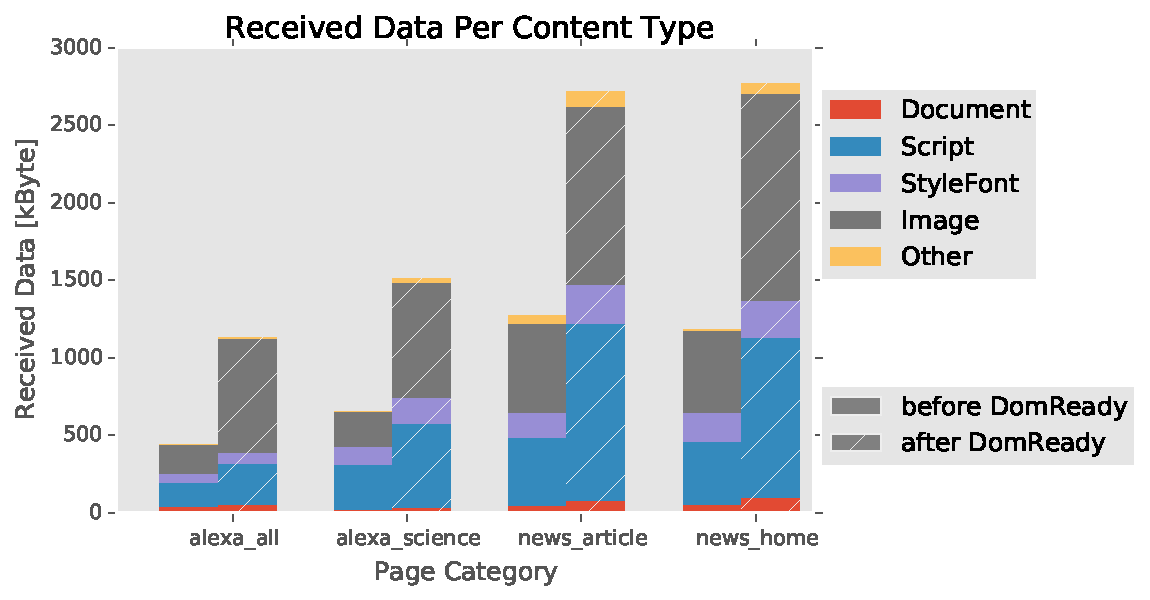
\includegraphics[width=0.7\textwidth]{wps-stackedSizeByCategory2.pdf}
	\caption{Transferred data for loading web pages, grouped by page category, 
	content type and relevance for DOM }
	\label{wps-stackedSizeByCategory2}
\end{figure}

\begin{figure}
\centering
	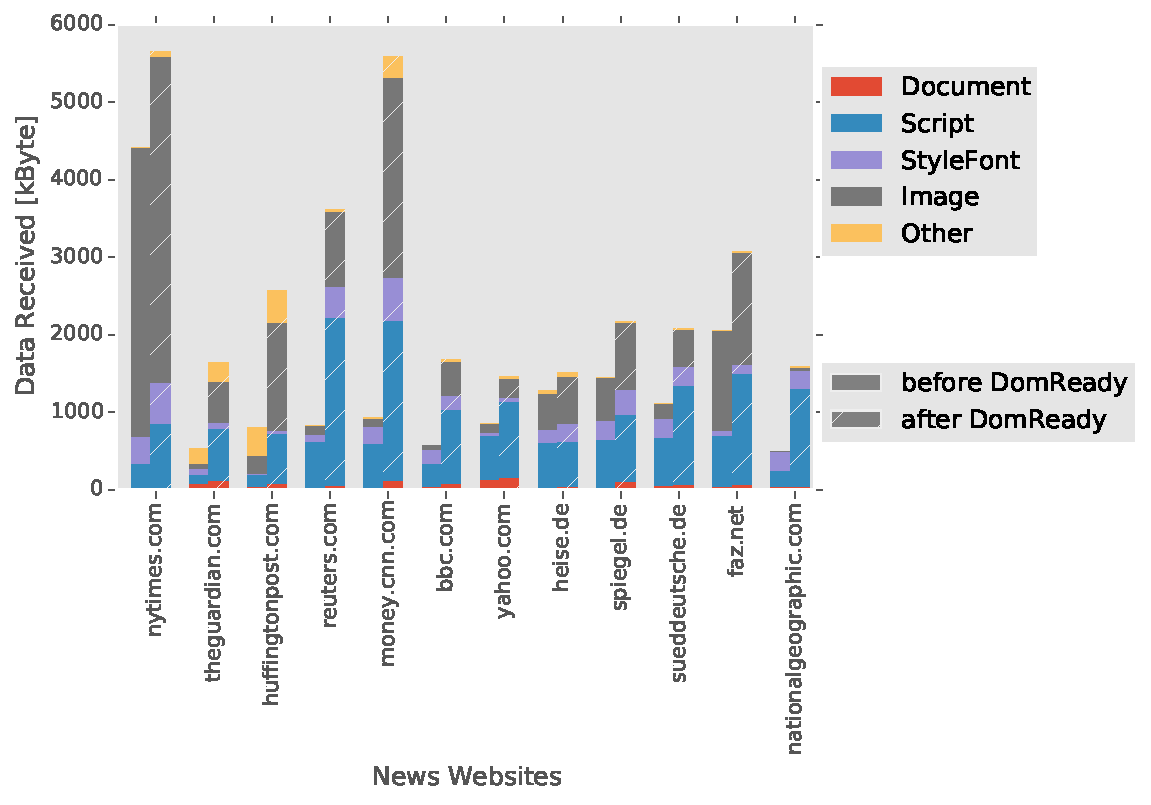
\includegraphics[width=0.8\textwidth]{wps-stackedSize-newsArticles.pdf}
	\caption{Transferred data for loading articles from different news sites, grouped by
	content type and relevance for DOM}
	\label{wps-stackedSize-newsArticles}
\end{figure}



In Figure \ref{wps-stackedSizeByCategory2} and \ref{wps-stackedSize-newsArticles} 
we plotted the transferred data on the Y axis, grouped by the request content 
types. In every block, the left bar shows the amount of data transferred 
before the DOMDocumentLoaded was fired, and the right bar the overall amount 
until the Load event.



\begin{figure}
\centering
	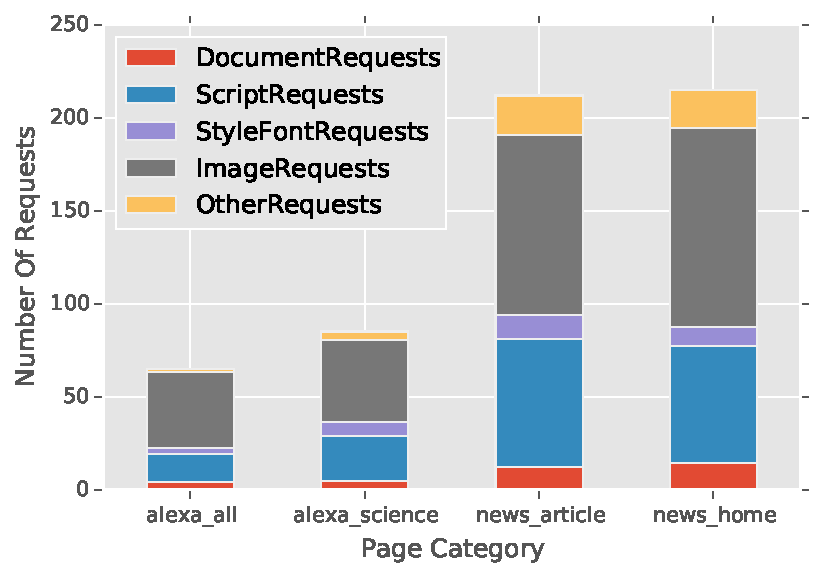
\includegraphics[width=0.65\textwidth]{wps-requestCountByCategory.pdf}
	\caption{Number of requests, grouped by page category, 
	content type and relevance for DOM }
	\label{wps-requestCountByCategory}
\end{figure}


We notice that in terms of received data, as well as number of request, the largest
portion of web pages is made up by scripts and images. 
The differences in received data before and after DOM is ready shows us candidates for
scheduling optimizations: For example, a majority of images are loaded after the DOM is ready,
allowing us to prioritize them lower without delaying DOM ready event. On the other hand,
the document is naturally needed for building the DOM tree, and also 85\% of style sheets 
are loaded before DOM ready. Therefore, prioritizing them higher could lead to faster
DOM ready times. The same is true for part of the scripts: usually, scripts which
are relevant to the page content, are referenced in the header of the page, making the DOM
ready depend on them, whereas tracking and similar scripts are often loaded asynchronously,
so, they are loaded afterwards.

%\todo{???????????????????????}


Interesting is also the difference in page size between the overall top sites 
and newspaper sites, especially regarding images. This can be partially 
explained by the fact that half of the top sites are search engine and social 
network home pages, containing only a search box or a login form, 
respectively, whereas the newspaper home pages are long illustrated lists of 
news article teasers.
On the other hand, the Alexa overall top sites are, with few exceptions, 
heavily optimized for minimum page size, whereas newspaper sites tend to 
include a huge amount of third-party JavaScript for advertising. This is also 
reflected in the amount of origins the resources are fetched from, as 
visualized in Figure \ref{wps-originCountByCategory}. On average, 73\% of 
requests where third-party requests.

\begin{figure}[h]
\centering
	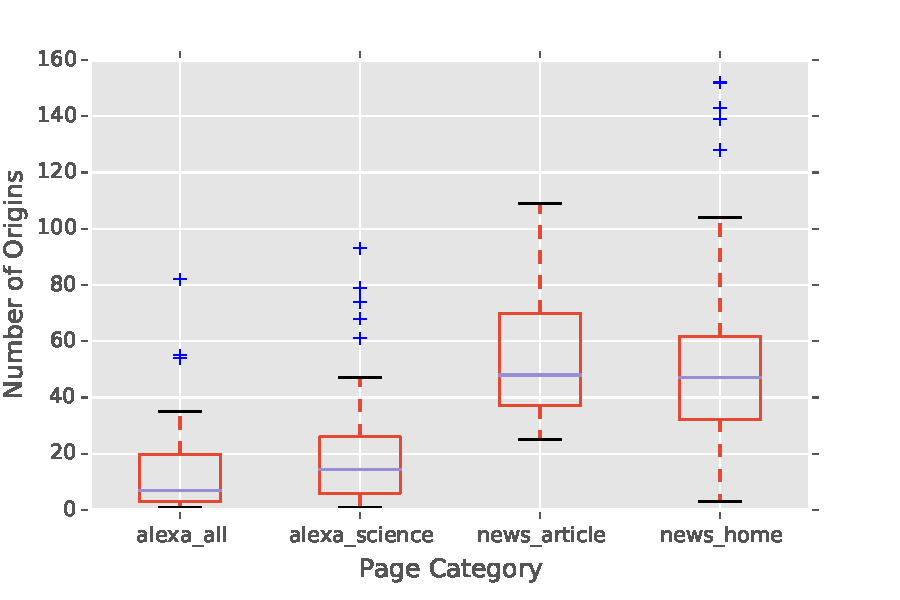
\includegraphics[width=0.65\textwidth]{wps-originCountByCategory.pdf}
	\caption{Number of request origins, group by page category}
	\label{wps-originCountByCategory}
\end{figure}



\clearpage

\begin{figure}
	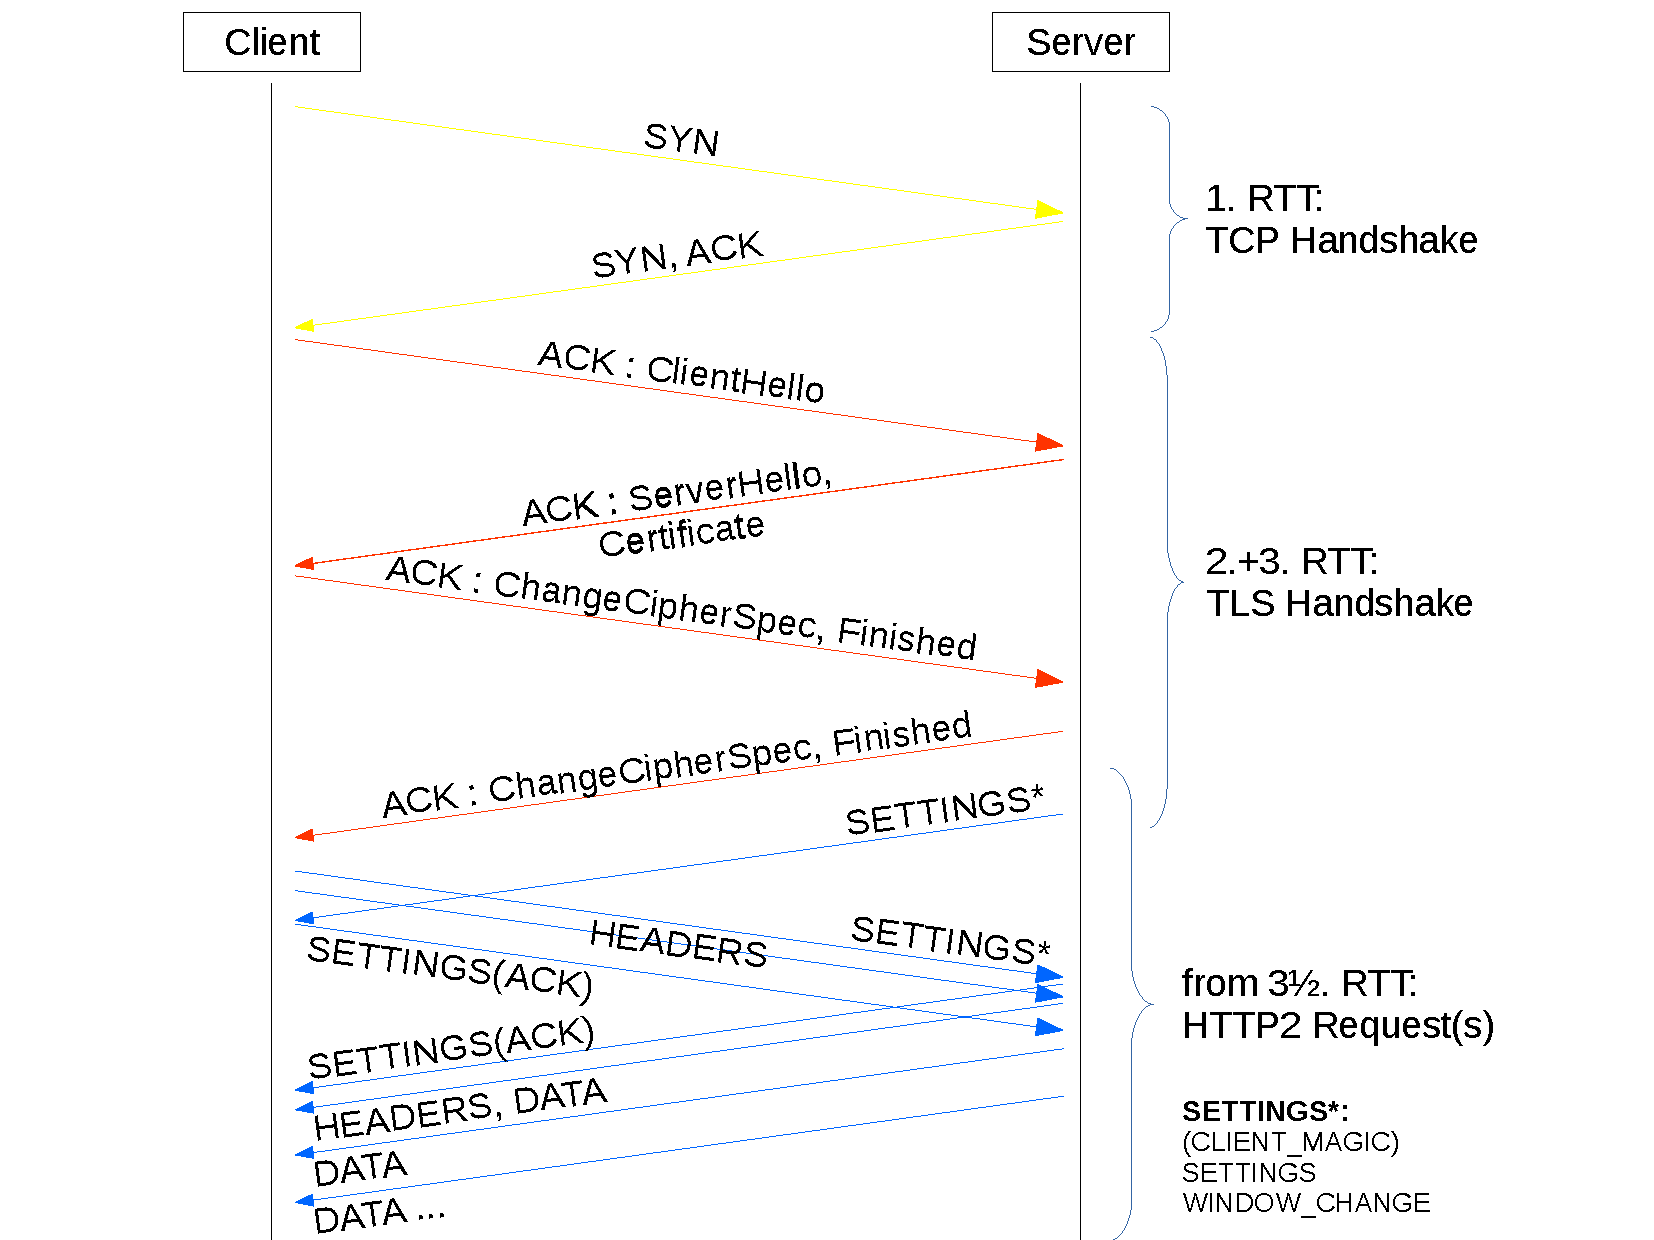
\includegraphics[width=1\textwidth]{http2_flow.pdf}
	\caption{TCP, TLS and HTTP/2 connection setup flow}
	\label{http2_flow}
\end{figure}


\section{Interaction between Transport and Application Layer} \label{approach-interaction}

%%%%%%%%%%%%%%%%%%% moved from background %%%%%%%%%%%%%%%%%%%%%
%% technical problems to be solved:
%% *api needs to be defined
%% *there might be a layer in between (Presentation Layer, TLS omnipresent today)

%There are two main technical challenges in cooperation between (network) layers:

%The first is that an adequate API needs to be defined. This is tricky especially in our case, the cooperation of application and transport layer, as one side is in user space and the other is a kernel component in modern operating systems.

%The second challenge results from the fact that these layers are not directly adjacent to each other: In our case it is TLS encryption, which operates in the presentation layer, making all application layer data opaque to layers below. Therefore, a side channel needs to be established to allow information flow around the TLS encryption.
%% see also: security considerations...
%%%%%%%%%%%%%%%%%%% ENDE moved from background %%%%%%%%%%%%%%%%%%%%%




%Wie dem Scheduler mitteilen was er tun soll?
%Problem: Wie erfolgt Kommunikation mit dem mptcp-scheduler? Zwischen mptcp und http2 sitzt in der regel noch tls! -> Paketinhalt f�r mptcp-scheduler nicht lesbar - evtl. �ber byte-counter


%Wo kommt die Logik hin?
%	- a: Server taggt Frames irgendwie, z.B. Inhalt=PageContent / Bild / Script / Style; Push=Ja/Nein; etc�, und Scheduler enth�lt die Logik die sagt was mit welchem Frame-Typ passieren soll
%oder b: Server gibt genaue Anweisung an Scheduler, dieser setzt es nur um
A decision we need to make is where to place the optimization logic. One 
approach is that the server tags every HTTP/2 frame with information like 
content or stream type, and the scheduler script decides that to do exactly. 
This way, there is maximum flexibility for the MPTCP configuration and the 
server doesn't need to know very much about MPTCP. On the other hand, we need 
special handling on the scheduler level for every application protocol we 
want to optimize.
The other approach is to have several general scheduler algorithms, each with 
different performance trade-offs, while allowing the application to decide 
which scheduler algorithm should be enabled. This reduces the dependencies on 
the scheduler level, but requires more MPTCP specific decision making on the 
application level. 

We take the former approach, where application specific hints are attached to 
the data stream, as it is passed down to the operating system. To pass the 
hints to the scheduler, we used a feature of the RBS. The application uses 
the \code{setsockopt} API call to set the hint for following data. It is 
valid until a different hint is set. Then, when the data is sent using the 
regular \code{write} call, the TCP stack records the current hint as metadata 
of the socket kernel buffer the data is stored in. 




\section{Optimizing the Multipath TCP scheduler}

We consider several optimization approaches based on our analysis of web page structure and the approach to pass hints about content and priority to the scheduler.


\subsection{Switching the Scheduler Based on Content Type or Priority}

Many modern web pages consist of dozens of resources. They can be classified 
by their technical priority for rendering the page. We described the resource 
content types in section \ref{request-content-types}. 
Modern browsers and speed-optimized web pages make sure that the resources 
with the highest technical priority are requested first. The HTTP/2 server 
can also facilitate this by pushing out high-priority resources with HTTP Push.

We can also look at the subjective utility as perceived by the user: In the 
case of text heavy pages, like on news sites, the Document and some images 
are most useful to the user as that contains the content of the page. In 
these cases, the JavaScript resources are often providing tracking and 
advertising. They are very important for the web site operator but not useful 
(even annoying) for the user. Especially tracking scripts can be delivered 
with lower priority as they are invisible and not time critical. On the other 
hand, for single page web applications and other interactive pages all the 
relevant content is loaded by JavaScript. Therefore, JavaScript resources 
have a high user utility here.

Therefore, we can try to single out resources with low technical priority and 
low subjective utility. By giving this as a hint to the scheduler, these 
might be transmitted only on a cheaper but slower subflow. On the other hand, 
the higher prioritized contents could be transmitted redundantly in case of a 
lossy connection.
The resources with high technical priority, especially if required for the 
first layout cycle, will be handled by a scheduler with emphasis on low 
latency. 
%
%latency critical stuff -> redundant if lossy
In case of a lossy connection, this could be a scheduler transmitting packets 
redundantly on all subflows, thereby minimizing delays caused by packet loss.
%latency critical stuff -> send on backup if backup has lower rtt
%\todo{...or send on low-rtt despite IS\_BACKUP}
%-> combine by checking for loss+rtt
After these high priority resources are sent out, a more bandwidth conserving 
scheduler can be used. For example, if one subflow has a higher cost than the 
other, we could prevent lower priority resources from being sent over this 
expensive path.



\subsection{Aggressive Transmission of Last Segments} \label{optimization-aggres-last-seg}
The transmitting application signals the state of its outgoing buffers to the scheduler. An interesting condition occurs when the HTTP server has no more data to send, and only a few segments are left in the scheduler's queue. This means only these few segments are missing so that a complete web page can be rendered for the user. The scheduler can try to push out the missing segments more aggressively: By temporarily ignoring the available congestion window for the left-over bytes, or by retransmitting on all available subflows.





\section{Security Considerations}
The information passed from the HTTP server to the MPTCP scheduler creates a side channel bypassing TLS encryption. It needs to be considered whether the passed data or the observable scheduler decisions based on this data could help an adversary. Some information is only protected by HTTP/2 and would be exposed on HTTP/1.1 connections anyway, like the length of individual resources. Others, like the content type, might be not available to the attacker otherwise. Therefore, content-type aware schedulers should be used only if the knowledge about the composition of the downloaded web site is not considered security critical information.






%=====================================================================
\chapter{Implementation}
%==============================================================================

For this work, we implemented and modified several pieces of software: (i) we 
adapted a web server to pass internal information to the kernel by setting TCP 
socket options; (ii) we 
implemented a Multipath TCP scheduler as RBS script which takes advantage of the 
hints given by the web server; (iii) we developed a set of scripts to instrument 
a web browser to load web pages, collect information about the process and 
aggregate it together with information from the operating system's network layer; 
(iv) we extended a framework for the evaluation of different Multipath TCP 
schedulers to run aforementioned client and server components.
This chapter contains the reasoning behind our 
choice of the web server to modify, as well as a detailed description of the 
implementation.

\section{Choosing a Web Server Platform}

Information about the contents of encrypted HTTP/2 application data is only 
available with cooperation of the web server. More precisely, we 
want to set socket options with hints for the scheduler, depending on 
information from higher levels. Multiple web servers have been evaluated and 
based on the criteria set out below, a suitable basis for the implementation 
has been selected.

To be considered, the server must support HTTP/2, and support it with at least 
one common browser as client. As we want to implement low-level modifications 
in the web server, the source code has to be available, and the license must 
permit modifications. This is a strictly necessary criterion, but luckily, most 
available web servers are permissively open source licensed under Apache, MIT 
or similar licenses. To make the work more relevant for practical use, a 
popular web server should be used. Therefore, we started our evaluation with 
Apache HTTP Server and NGINX, the two most popular open source HTTP servers. 
Apache HTTP Server internally uses the third-party library Nghttp2 for its 
HTTP/2 support, which contains the reference HTTP/2 server implementation 
Nghttpd, which we also evaluated and finally selected.


% NGINX (Plus)
% nginx has a open-source (community) and a ``enterprise'' version (NGINX Plus)
The \textbf{Nginx} web server is available as Open-Source Nginx and as the 
commercial, closed-source \textit{Nginx Plus}. Only the commercial edition 
has full HTTP/2 support, while the open-source ngx\_http\_v2\_module\footnote{%
\url{http://nginx.org/en/docs/http/ngx_http_v2_module.html}} lacks the 
``Server Push'' feature.
% only NGINX Plus has full HTTP/2 support, in the open source version e.g., no http2 push is supported


% Apache HTTP Server
% bucket brigades are too complicated...
The \textbf{Apache HTTP Server} fully supports HTTP/2 with its mod\_http2 
module. The module is based on Nghttp2, an HTTP/2 C library. We investigated 
the inner workings of Apache HTTP Server, following the byte stream from 
libnghttp2 to OpenSSL and finally the TCP socket. These internals are based on 
the Apache Portable Runtime\footnote{\url{https://apr.apache.org/}} (APR) and 
the concepts of Filters, Buckets, and Bucket Brigades.  To implement our 
extension, we would have to add additional metadata to every Bucket, making 
sure, that it isn't lost in intermediate Filters. Another possibility is to add 
a new type of metadata buckets\footnote{%
\url{https://httpd.apache.org/docs/trunk/developer/output-filters.html}}, 
inserting them between data buckets every time the metadata (e.g. content type) 
changes.

% Nghttpd
Aside from the library, the Nghttp2 project also provides reference client, 
server and proxy implementations. Their server, \textbf{Nghttpd}, promised to 
be much less complex than Apache, while being still based on the same library. 
It has only one layer of buffering between the ``output'' of libnghttp2 and 
\code{SSL_write}, the ``input'' of OpenSSL, making it easy to pass along 
metadata. Also, the whole server consists of just over 3000 total lines of 
C++ code. This led us to use Nghttpd as the basis for our implementation.

 



\section{Modifications to the Web Server}

Figure \ref{fig:annotated-data-path} visualizes the way an HTTP request takes
through the different components of the Nghttpd web server. 
First, the data is read from OpenSSL and pushed into the Libnghttp library 
as described in section \ref{nghttpd-streamctype}. This can be seen in the
lower left of the figure. In the top two rows, the internal logic which resolves
an HTTP URL to a file is only schematically indicated.
The part in the middle, pointing into the ``opaque octet buffer'' are described in
Section \ref{nghttpd-retr-meta-inf}, whereas the output from said buffer is 
described in Section \ref{nghttpd-passing-meta}.

Nghttpd uses libev for managing its control flow, an event loop library, which means the 
program is structured in several event watcher functions, called from the 
main loop, when, for example, data is available or can be sent through a 
network socket, or when a timeout is reached. 

\begin{figure}
	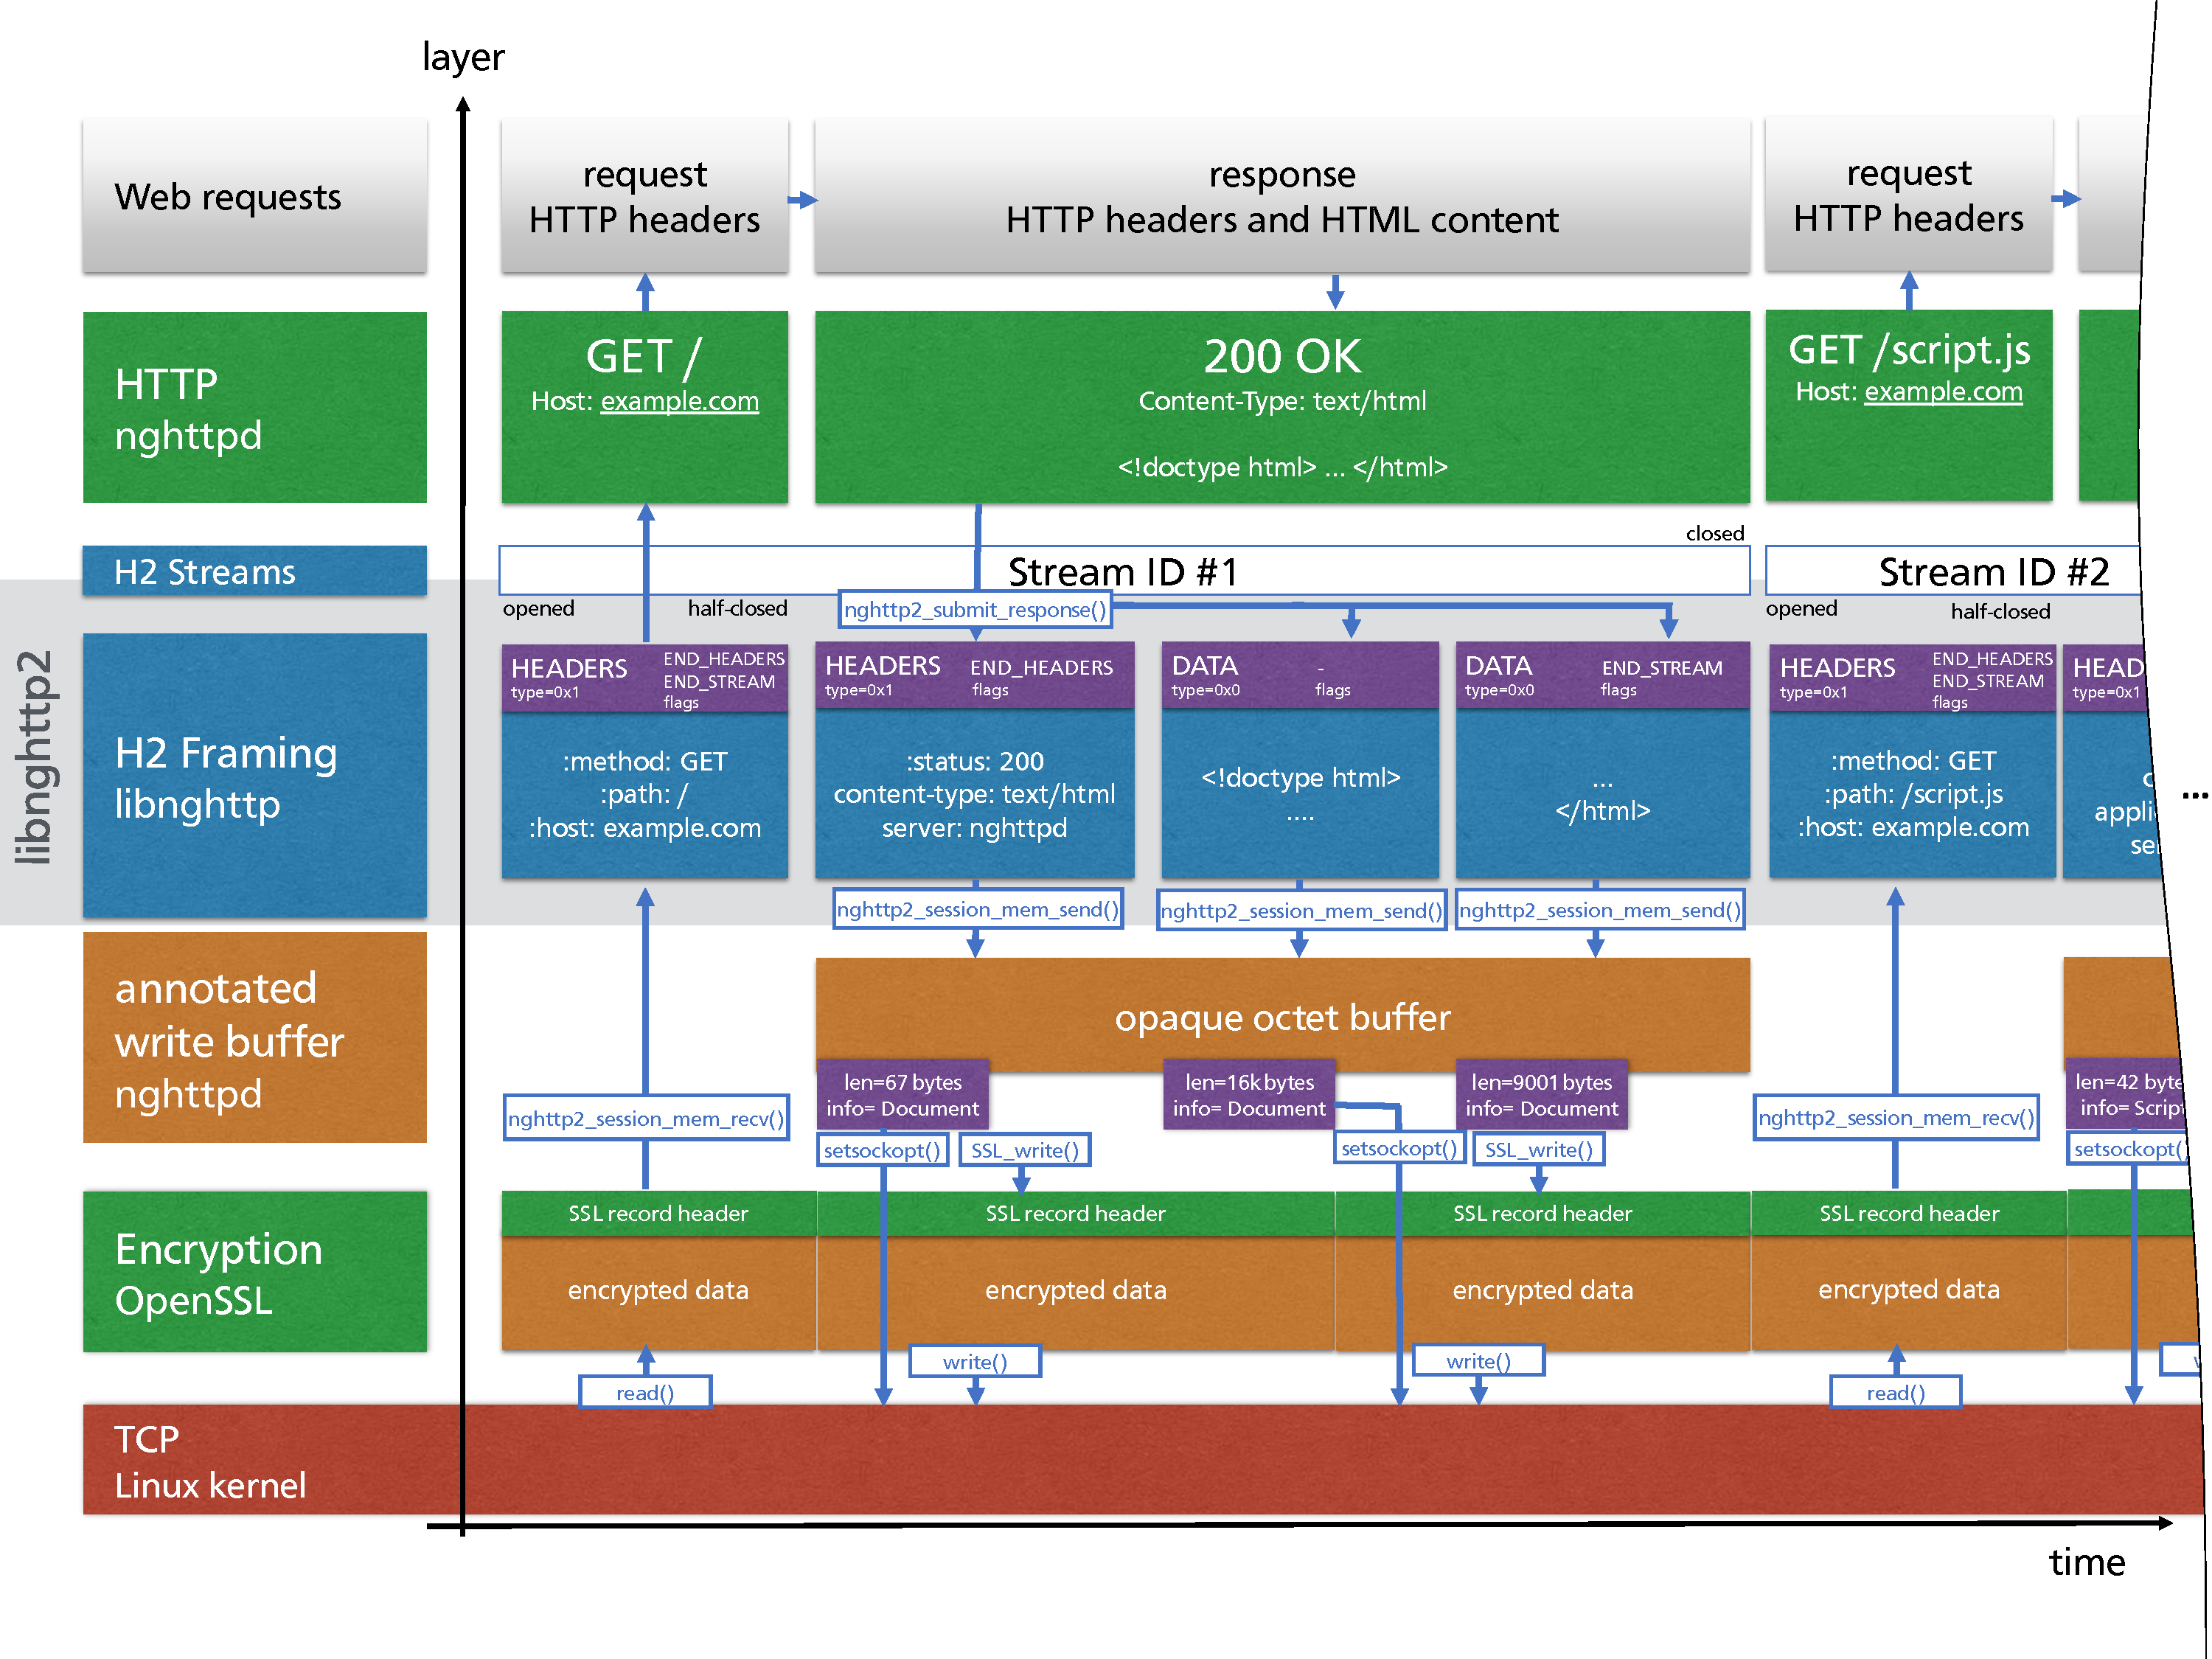
\includegraphics[width=1\textwidth]{nghttpd-data-flow.pdf}
	\caption{The annotated data's path through the Nghttpd web server}
	\label{fig:annotated-data-path}
\end{figure}


\subsection{Initializing RBS Scheduler}
One of these event watchers is \code{accept_connection}, which is called when 
a new client connects. It creates a new instance of the \code{Http2Handler} 
class, which, among other things, registers its \code{read_tls} and \code{
write_tls} methods to be called when new data is received from the client or 
can be sent out, respectively. We extend the connection setup code as shown 
in Listing \ref{lst:nghttpd-select-ruleset} to select a RBS scheduler. This 
is done via a special \code{setsockopt} call and is valid for the current 
socket. The scheduler to select is configured via the command line argument 
\texttt{-{}-mptcp-ruleset}.


% selecting a RBS script for HTTP/2 connections (command line parameter)
\begin{lstlisting}[style=C_Code,label={lst:nghttpd-select-ruleset},caption={The extended Nghttpd connection setup method (from \code{HttpServer.cc})},numbers=left,firstnumber=281,linebackgroundcolor={\lstLinesAdded{284-295}}]
  void accept_connection(int fd) {
    util::make_socket_nodelay(fd);

#ifdef MPTCP_DEBUG
    printf("MPTCP: Selecting ruleset \"%s\" ...\n", config_->mptcp_ruleset.c_str());
#endif
    if (config_->mptcp_ruleset.length() != 0) {
      // configure MPTCP rule-based scheduler ruleset
      if (setsockopt(fd, IPPROTO_TCP, MPTCP_RULE_SET, config_->mptcp_ruleset.c_str(), 
			config_->mptcp_ruleset.length()) < 0) {
        perror("Error: Could not select ruleset for socket");
        close(fd);
        return;
      }
    }

    SSL *ssl = nullptr;
    if (ssl_ctx_) {
      ssl = ssl_session_new(fd);
      if (!ssl) {
        close(fd);
        return;
      }
    }
    auto handler =
        make_unique<Http2Handler>(this, fd, ssl, get_next_session_id());
    if (!ssl) {
      if (handler->connection_made() != 0) {
        return;
      }
    }
    add_handler(handler.release());
  }
\end{lstlisting}

\subsection{Recording the Content Type of Streams} \label{nghttpd-streamctype}
\code{read_tls} reads data from the socket via OpenSSL's \code{SSL_read} 
function, and calls \code{nghttp2_session_mem_recv}, a library function of 
Libnghttp. The library parses the incoming data, and informs the main server 
code of any new requests over a callback. 

% each HTTP/2 request is internally a Stream (in spec+server)
% store information about/in the stream: simplified content type -> priority
According to the HTTP/2 protocol specification each new request is processed 
in a separate stream. Accordingly, Nghttpd has a \code{Stream} structure 
which is instantiated for each request and stores relevant information. We 
extend this class as shown in Listing \ref{lst:nghttpd-struct-stream} by a 
\code{scheduling_content_type} field, which is a simplified representation of 
the response's content type. The possible values of this field are declared 
in Listing \ref{lst:scheduling-content-type-decl}.

\begin{lstlisting}[style=C_Code,label=lst:nghttpd-struct-stream,caption={
	The extended Nghttpd \code{Stream} structure (from \code{HttpServer.h})
},numbers=left,firstnumber=142,linebackgroundcolor={\lstLinesAdded{156-157}}]
struct Stream {
  BlockAllocator balloc;
  RequestHeader header;
  Http2Handler *handler;
  FileEntry *file_ent;
  ev_timer rtimer;
  ev_timer wtimer;
  int64_t body_length;
  int64_t body_offset;
  // Total amount of bytes (sum of name and value length) used in
  // headers.
  size_t header_buffer_size;
  int32_t stream_id;
  bool echo_upload;
  // simplified content type, can be used as mptcp scheduler hint
  uint32_t scheduling_content_type;
  Stream(Http2Handler *handler, int32_t stream_id);
  ~Stream();
};
\end{lstlisting}


% content type 
The response to a request is generated in \code{prepare_response}. There, the 
request URL is parsed to find the file which should be delivered to the 
client. We extended this with primitive mechanism for categorizing file types 
based on the file extension, as well as a query string parser. The query 
parameter \code{rbs_content_type} allows overriding the automatically 
assigned file type. Finally, the response is enqueued in Libnghttp's internal 
buffer of outbound items by calling \code{nghttp2_submit_response}. The 
modifications are reproduced in Annex \ref{annex-prepare_response}.

\subsection{Retrieving and Buffering Meta Information} \label{nghttpd-retr-meta-inf}

The event watcher \code{write_tls} is run whenever the socket signalizes that 
data can be sent out. It serves two purposes: if data to be sent is available 
in \code{wb_}, it sends it out over OpenSSL's \code{SSL_write}. \code{wb_} is 
an opaque buffer of octets, which means no information about the nature of the 
data inside is available at this point. It is used to decouple the generation 
of HTTP/2 encoded data by Libnghttp from the generation of TLS records by 
OpenSSL. If this wasn't done, each TLS record could contain at most a single 
HTTP/2 frame, which would be inefficient. If \code{wb_} is empty, 
\code{write_tls} runs \code{fill_wb}, which fetches outgoing data from 
\code{nghttp2_session_mem_send}, and enqueues it in \code{wb_}. We extend this 
process with a FIFO implemented as a linked list as declared in Listing 
\ref{lst:nghttpd-linkedlist-headers}. The FIFO stores metadata about the 
octets enqueued in \code{wb_}, along with the number of octets this metadata 
is valid for. 

\begin{lstlisting}[style=C_Code,label=lst:nghttpd-linkedlist-headers,caption={
Declaration of the data structure for metadata storage (from \code{mptcp_rbs.h})}]
struct skb_prop_range {
  struct skb_prop_range* next;
  unsigned int frameLength;
  unsigned int skbProperty;
};

unsigned int skb_prop_peek(struct skb_prop_range **list);
void skb_prop_pop(struct skb_prop_range **list, unsigned int bytes);
void skb_prop_push(struct skb_prop_range **list, unsigned int bytes, unsigned int skbProp);
\end{lstlisting}

\code{fill_wb} enqueues and \code{write_tls} dequeues the 
metadata in lockstep with the data. In Listing \ref{lst:nghttpd-fill_wb} the 
code for enqueueing the meta information is highlighted. There is a second
function where data and metadata are enqueued, which is the 
\code{send_data_callback}. It is used as a performance optimization to avoid 
unnecessary data copy in memory. For our purposes, it can be viewed as
identical to \code{fill_wb}.


\begin{lstlisting}[style=C_Code,label=lst:nghttpd-fill_wb,caption={
	Fetching and forwarding data and meta data (from 
	\code{HttpServer.cc}, method \code{Http2Handler::fill_wb})
},linebackgroundcolor={\lstLinesAdded{11-13,15-16}}]
    const uint8_t *data;
    // pick up some data from nghttp2's outbound item queue
    auto datalen = nghttp2_session_mem_send(session_, &data);
    [...]
    // enqueue the data in the write buffer
    auto n = wb_.write(data, datalen);
    [...]
    // get meta information about the data block
    unsigned int mySkbProp = get_skb_property(
	    get_config(), FROM_FILL_WB, &session_->aob.item->frame, stream);
    // store the meta information, noting it is valid for the next 'datalen' octets
    skb_prop_push(&skbProp, datalen, mySkbProp);
\end{lstlisting}




The metadata is provided by the function \code{get_skb_property} in Listing 
\ref{lst:nghttpd-get_skb_property}. A command line parameter is used to 
configure what information to use as the hint. With our optimized scheduler 
scripts, the \code{scheduling_content_type} is used, therefore mptcp-skb-prop 
should be set to \code{RBS_PROP_CONTENTTYPE}. For testing, we added other 
types of hints, like a counter which is incremented at every call to the 
function, and the type of HTTP/2 frame (see Section \ref{http2-frame-types}).

\begin{lstlisting}[style=C_Code,numbers=left,label=lst:nghttpd-get_skb_property,caption={
The \code{get_skb_property} function added to Nghttpd (from \code{HttpServer.cc})}]
592  unsigned int get_skb_property(const Config *config, int caller, nghttp2_frame *frame, Stream *stream) {
593    testCounter += 1;
  [...]
602    switch(config->mptcp_skb_property_mode) {
603      case RBS_PROP_CONTENTTYPE:
604        if (!stream) return SKB_CONTENT_NOSTREAM;
605        return stream->scheduling_content_type;
606      case RBS_PROP_COUNTER:
607        return testCounter;
608      case RBS_PROP_FRAMETYPE:
609        if (!frame) return 0;
610         return frame->hd.type;
	[...]
614    }
615  }
\end{lstlisting}


\subsection{Passing Meta Information to the Multipath TCP Scheduler} \label{nghttpd-passing-meta}

% setting scheduling hints as RBS_USER socket option

To provide our meta information to the Multipath TCP scheduler as scheduling 
hints, we use the socket option API. As suggested above, \code{write_tls} 
sends out data from the write buffer to OpenSSL whenever the socket 
signalizes that data can be sent out. Before doing so, it relays the current 
meta information from the FIFO to the TCP stack. Only after writing out the 
data we can be sure how many octets were really written. Then we remove this 
number of octets from the write buffer and from the metadata FIFO. This is 
implemented by the code in Listing \ref{lst:nghttpd-write_tls-metarelay}.

\begin{lstlisting}[style=C_Code,label=lst:nghttpd-write_tls-metarelay,caption={
Relaying metadata (from \code{HttpServer.cc}, method \code{Http2Handler::write_tls})}]
      // relay metadata from FIFO to OS
      rbs_set_skb_property(fd_, skb_prop_peek(&skbProp));
      [...]
      auto rv = SSL_write(ssl_, wb_.pos, bytesToWrite);

      if (rv <= 0) {  // handle errors
        [...]
      }
      // drain metadata and data FIFOs
      skb_prop_pop(&skbProp, rv);
      wb_.drain(rv);
\end{lstlisting}

Another information we provide to the RBS scheduler is whether we have more
data in our internal buffers. This can be used for optimizations as described 
in Section \ref{optimization-aggres-last-seg}. In Nghttpd, data can be buffered
in the outgoing item queue of Libnghttp, and in the octet write buffer \code{wb_}
of the Http2Handler class. We set the register \textbf{R1} to \texttt{1} if both
queues are empty, and to \texttt{0} otherwise. 

\begin{lstlisting}[style=C_Code,label=lst:nghttpd-write_tls-bufferstate,caption={
Informing RBS about our buffer state (from \code{HttpServer.cc}, method 
\code{Http2Handler::write_tls})}]
set_rbs_register(1,  // register R1
				 (skbProp == NULL && nghttp2_session_want_write(session_) == 0) ? 1 : 0);
\end{lstlisting}

A similar approach would be to store the current buffer size in this register. However, only the size of the write buffer (\code{wb_}) is known at this point, whereas the ``outbound items'' queued in the nghttp2 library are quite unpredictable since items can contain a callback function pointer, which, when called, produces the actual data.



\subsection{TLS Record Size}

% changing the maximum ssl record size
As explained in Section \ref{tls-background}, we were concerned with TLS 
record sizes and boundaries. We therefore added the 
\texttt{-{}-max-ssl-record-size} command line option to Nghttpd. This allows 
us to modify the maximum size of TLS records. This is implemented by capping 
the maximum number of bytes to write which is specified when calling 
\code{SSL_write} from the \code{Http2Handler::write_tls} method.

\begin{lstlisting}[style=C_Code,caption={
Limiting the number of bytes in a TLS record (from \code{HttpServer.cc}, 
method \code{Http2Handler::write_tls})}]
      auto bytesToWrite = wb_.rleft();
      if (bytesToWrite > get_config()->max_ssl_record_size)
			bytesToWrite = get_config()->max_ssl_record_size;
      auto rv = SSL_write(ssl_, wb_.pos, bytesToWrite);
\end{lstlisting}






%\clearpage

\section{Combining Nghttpd and RBS Schedulers} \label{nghttpd-query-params}

Our extended version of Nghttpd supports additional command line arguments 
and query string parameters to make use of Rule-Based Scheduler features. 

\subsection{Command Line Arguments}

Multiple scheduler scripts can be loaded in the RBS at the same time. To select 
which one to use for HTTP/2 connections, the argument \texttt{-{}-mptcp-ruleset=\textit{<name>}}
must be supplied. Its value should be the name of a loaded scheduler as listed 
in \code{/proc/net/mptcp_net/rbs/schedulers}.

Consistent with the scheduler, we need to configure which kind of metadata 
Nghttpd will supply. Valid metadata indices for the 
\texttt{-{}-mptcp-skb-prop=\textit{<index>}} argument are shown in Listing 
\ref{rbs-prop-indizes}.

\begin{lstlisting}[style=C_Code,label=rbs-prop-indizes,caption={
Constants defining valid metadata indizes (from \code{mptcp_rbs.h})}]
#define RBS_PROP_COUNTER       0    /* counter incremented at every HTTP/2 frame (part) */
#define RBS_PROP_FRAMETYPE     1    /* frame type as defined in HTTP/2 standard */
#define RBS_PROP_STREAMID      2    /* stream identifier (unique per connection), mod 255 */
#define RBS_PROP_CONTENTTYPE   3    /* simplified content type as defined in SKB_CONTENT_* constants */
\end{lstlisting}

\subsection{URL Query Parameters}

The scheduler hints can be augmented by the following parameters in the URL 
query string (``GET parameters''). The code parsing these parameters can be 
found in Annex \ref{annex-prepare_response}.

When we use existing web pages for measurements, the content types of requests often can't be determined by the file extension. Therefore, we implemented the \code{rbs_content_type} parameter which we can add to the URLs in the code of the downloaded web page to override
the content type which is used as a scheduler hint. Valid types can be found 
in Listing \ref{lst:scheduling-content-type-decl}.

For testing purposes, it proved useful to be able to set the internal 
registers of the RBS script via the \texttt{rbs\_set\_R\textit{<n>}} 
parameter. The register number and values depend on the individual scheduler 
script. For example, before we had implemented content type hints, we used this feature to explicitly specify a segment number offset at which the scheduler algorithm should be switched. 
Register R1 can't be used with this parameter as it is used for 
the buffer state information, and therefore would be overwritten directly (c.f. Listing \ref{lst:nghttpd-write_tls-bufferstate}).



\subsection{Scheduler Registers and USER Field}

We can use the \code{<packet>.USER} property and registers R1 to R6 as set by 
the application code to select the scheduling algorithm or optimize 
scheduling preferences. With the following explanation and listings, we 
document and provide examples how the scheduling hints can be used in the RBS 
script.

As the USER field is a numeric value, we need to settle on a mapping between 
content types and numbers understood by application and transport layer. All 
content-aware scheduler scripts contain this mapping as the block of 
definitions in listing \ref{lst:scheduling-content-type-decl}.

\begin{lstlisting}[style=RBS,label=lst:scheduling-content-type-decl,caption={
Possible values of the USER field if simplified content types are used as hints}]
VAR SKB_CONTENT_NOSTREAM =  1;   /* data is not part of a stream */
VAR SKB_CONTENT_DOCUMENT =  2;   /* .html .htm */
VAR SKB_CONTENT_SCRIPT   =  3;   /* .js */
VAR SKB_CONTENT_STYLE    =  4;   /* .css */
VAR SKB_CONTENT_IMAGE    =  5;   /* .jpg .png .gif */
VAR SKB_CONTENT_OTHER    =  6;   /* all other filetypes */
\end{lstlisting}



To test the implementation of content-type specific scheduling, we can mark a 
fast subflow as \textit{backup}, which usually means 'not to be used as long 
as other subflows are available'. We then provide the scheduler in listing 
\ref{lst:ctype-based-subflow-filter}, which won't transfer any images on the 
backup subflow, but will still consider it for other content types.

\begin{lstlisting}[style=RBS,label=lst:ctype-based-subflow-filter,caption={
Filtering usable subflows based on content type from USER field}]
/* next SKB is marked as image content? */
IF (Q.TOP.USER == SKB_CONTENT_IMAGE) {
    /* the subflows marked as "BACKUP" are filtered out */
    usableSbfs.FILTER(sbf => !sbf.IS_BACKUP).MIN(sbf => sbf.RTT).PUSH(Q.POP());
} ELSE {
    /* all available subflows are used */
    usableSbfs.MIN(sbf => sbf.RTT).PUSH(Q.POP());
}
\end{lstlisting}

Another way to use content type information, especially in network situations 
with high packet loss, is to send latency-critical data redundantly. 
We should consider all data not belonging to a stream as critical, because it 
is the TLS handshake and a few HTTP/2 settings frames at the start of the 
connection. In the example listing \ref{lst:ctype-based-redundancy} we also 
consider the document as critical, because it contains the text contents of 
the page as well as references to all other elements, whereas we don't add 
scripts here, because they are often a large percentage of overall page size 
(c.f. Analysis of page structure in Section \ref{page-structure-findings}). A 
better approach could be to consider scripts only critical if required for 
the First Contentful Paint of the page.

\begin{lstlisting}[style=RBS,label=lst:ctype-based-redundancy,caption={
Sending packets redundantly based on the content type from USER field}]
/* next SKB is document or non-stream data? */
IF (Q.TOP.USER <= SKB_CONTENT_DOCUMENT) {
    /* critical packet, send redundantly */
    FOREACH(VAR sbf IN usableSbfs) {
        sbf.PUSH(Q.TOP);
    }
    DROP(Q.POP());
} ELSE {
    /* otherwise, send it only on fastest subflow */
    usableSbfs.MIN(sbf => sbf.RTT).PUSH(Q.POP());
}
\end{lstlisting}

As we are informed about the queue levels of the application over the R1 
register, we can use this information for scheduling decisions as well.
For example, when our own \code{Q} sending queue is empty, and we know that 
no new data will come from the application soon, we can decide to retransmit 
unacknowledged packets on all subflows they haven't been sent on. This could 
speed up the ``tail'' of a connection, i.e. the last missing packets for 
displaying a web page. 

\begin{lstlisting}[style=RBS,label=lst:retrans-if-q-empty,caption={
Retransmitting unacknowledged packets if send queues are empty}]
VAR applicationQueuesEmpty = R1;
IF (Q.EMPTY && applicationQueuesEmpty == 1) {
    VAR usableSbfs = SUBFLOWS.FILTER(sbf => sbf.CWND > sbf.SKBS_IN_FLIGHT);
    
    /* resend the oldest packet which wasn't sent on all usable subflows yet */
    VAR oldestPacket = QU.
        FILTER(packet => 
            !usableSbfs.FILTER(sbf => ! packet.SENT_ON(sbf)).EMPTY
        ).TOP;
	
	/* retransmit only on subflows it has not yet been sent on */
    VAR newSbfs = usableSbfs.FILTER(sbf => !oldestPacket.SENT_ON(sbf));
	FOREACH(VAR sbf IN newSbfs) {
		sbf.PUSH(oldestPacket);
	}
}
\end{lstlisting}

%We use three timing metrics, which are available over the Chrome debugging protocol\footnote{\url{https://developer.chrome.com/devtools/docs/debugger-protocol}}, the protocol of the Google Chrome web browser's developer tools.

\clearpage
\section{Instrumenting the Web Browser} \label{measurement-script}

\begin{wrapfigure}{r}{0.6\textwidth}
	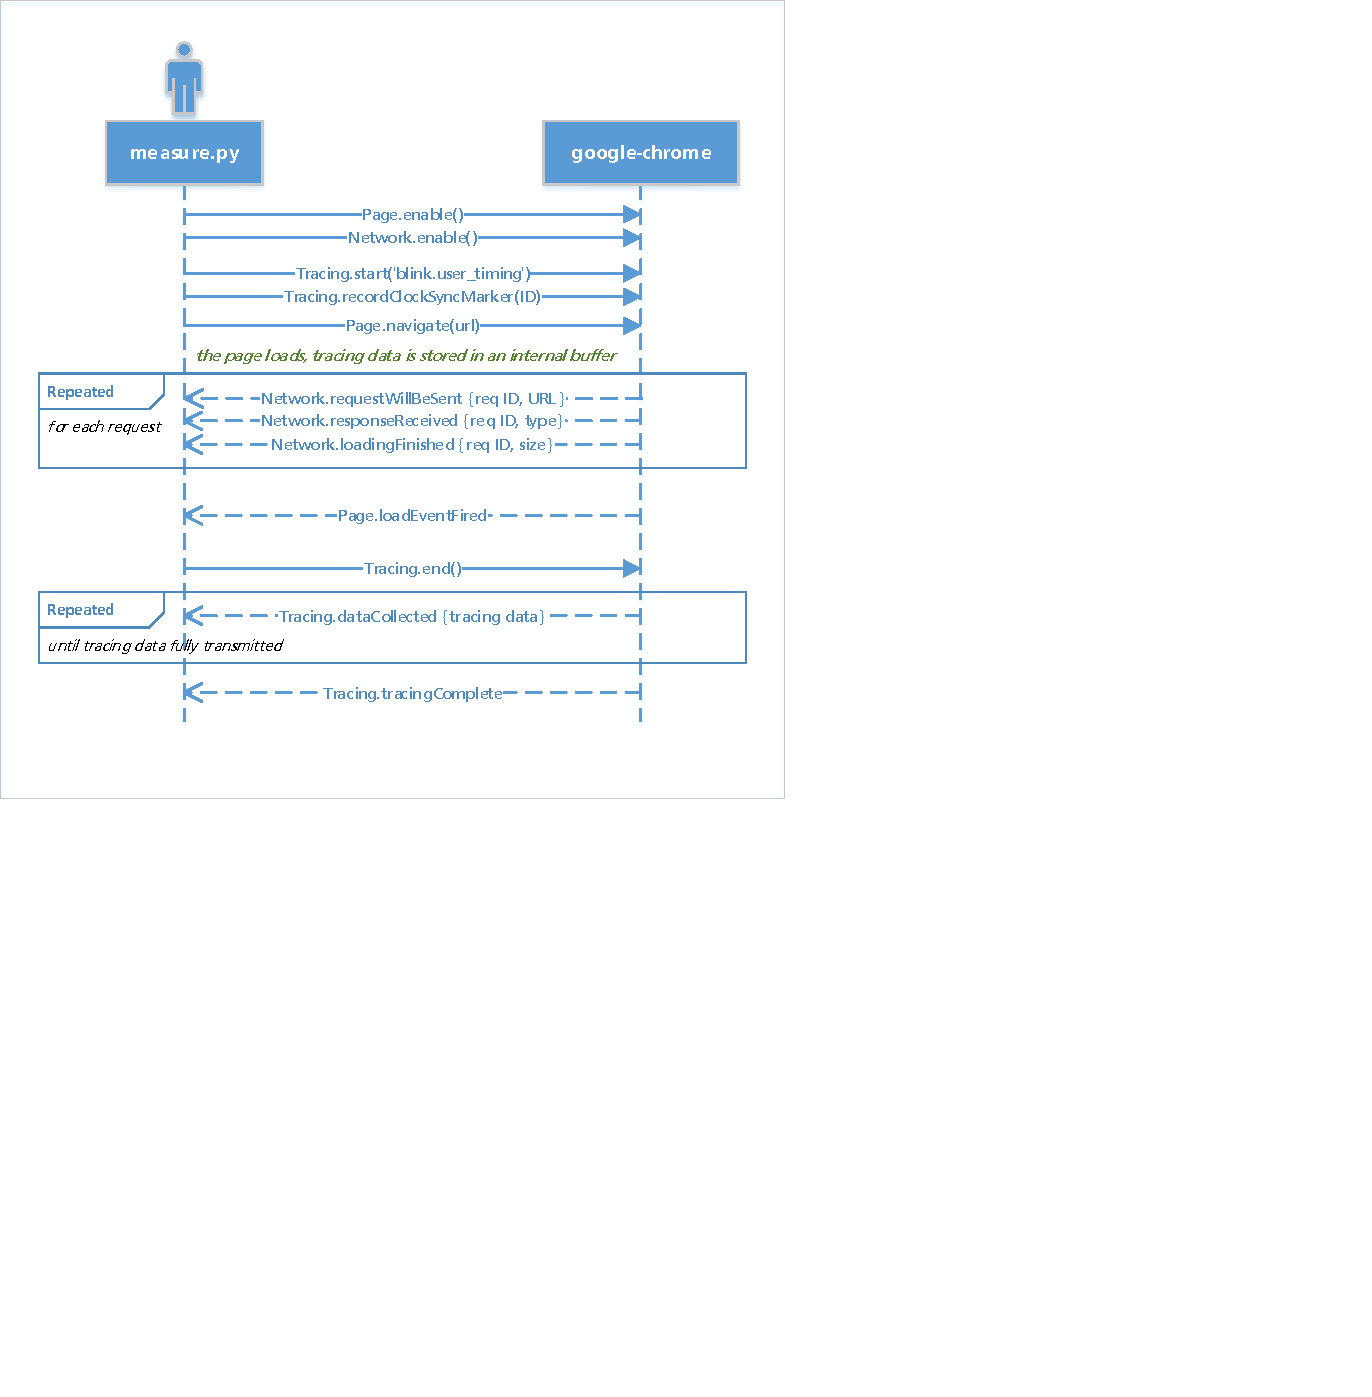
\includegraphics[width=0.6\textwidth, trim=0.25in 4.15in 4.15in 0.25in, clip]{chrome-tracing.pdf}
	\caption{A sample interaction with the Chrome Debugging API}
	\label{fig:chrome-tracing-api}
\end{wrapfigure}


In our analysis of web page structure, as well as in the later evaluations of 
collaborative schedulers, we use the timing metrics described in Section 
\ref{metrics-web-perf}. These are visible in the Google Chrome web browser's 
developer tools, however, it is necessary to collect and average the timings
of many page loads, because in a Mininet simulation the results can be 
influenced by multitasking effects, whereas in real networks transient delays 
and packet drops can occur on any middlebox along the route.  Therefore, we 
need to record them in an automated way, which is possible by directly 
connecting to the API the developer tools use internally, the Chrome 
Debugging Protocol\footnote{\url{https://developer.chrome.com/devtools/docs/debugger-protocol}}.
We built the Python script \code{measure_web_requests.py} to 
instrument the web browser to navigate to pages we want to measure, and to 
retrieve the network and tracing data.

A sample interaction with the browser over the Chrome Debugging Protocol is 
shown in Figure \ref{fig:chrome-tracing-api}. The script first starts a new 
Chrome instance with special parameters to prevent interference: we disable 
automatic updates, the popup blocker, welcome message, Google Translate, and 
others. We also specify a new profile directory, to prevent distortion from 
cached data from previous experiments. 

After connecting over the Chrome Debugging Protocol, it enables \textit{Page} 
and \textit{Network} related events and starts a new tracing session. Because 
the tracing API uses its own timestamps, we need to synchronize it with wall 
clock time first by calling \textit{recordClockSyncMarker}. This allows us to 
combine tracing API timings with network API timings later.
The script will then ask the browser to navigate to the page we want to 
measure. While loading, the tracing component of Chrome stores all events in 
an internal buffer. The network component sends us events of every resource 
load in real time. We accumulate the number of requests and the response sizes, 
grouped by origin (domain name and port) and by content type.

%note that we only measured requests before the onLoad event
%- usually web sites are finished with the onLoad event
%- e.g. google.com only starts loading its javascript after onLoad, but it is not necessary - site works without js
%- 
We stop the measurement when the Load event fires. This means all resources 
which are referenced in the document, even scripts with the \code{async} attribute, 
are, by definition, included. Requests finishing after the Load event fired, 
like AJAX requests, are not included in the results. Also, some websites that 
don't require JavaScript for their operation, e.g. the google.com homepage, 
only start loading their JavaScript after the Load event, causing it to be 
excluded from the result.

As a result, the script prints a report with tables of the tracing event timings
and request numbers and sizes.
A condensed version of the output is appended to a logfile in CSV format. The 
full results are also written to a machine-readable JSON file, which is then 
used by an aggregation script in the scheduler evaluation framework.

In the example report shown in Listing 
\ref{lst:measure-web-requests-output}, the English homepage of 
Wikipedia was loaded, which took 0.8 seconds in total. 310 kilobytes of data 
were transmitted from three different origins. 
In the second and third table, the column \texttt{\#req} shows the number of 
requests from this origin or of this type, respectively. 
The columns \code{xferAll} and \code{xferReady} give the kilobytes of data 
transmitted before the \textit{load} and before the \textit{DOMDocumentLoaded} 
event, respectively. The content types are listed in the third table. This 
allows us to see that document and stylesheets were fully loaded before the 
\textit{DOMDocumentLoaded} event, whereas most images loaded afterwards. 


%\clearpage
\begin{lstlisting}[label=lst:measure-web-requests-output,caption={
   A report generated by \code{measure_web_requests.py}
},keywords={},numbers=left,tabsize=8,escapeinside={(*}{*)}]
(*\aftergroup\bfseries*)URL: https://en.wikipedia.org/wiki/Main_Page
Timings:(*\aftergroup\mdseries*)
0.0000  navigationStart
0.0002  fetchStart
0.0842  unloadEventStart
0.0842  unloadEventEnd
0.0845  domLoading
0.1113  responseEnd
0.2112  domInteractive
0.2112  domContentLoadedEventStart
0.2112  domContentLoadedEventEnd
0.3612  firstLayout
0.3708  firstPaint
0.3708  firstTextPaint
0.3708  firstContentfulPaint
0.3708  firstImagePaint
0.7463  domComplete
0.7464  loadEventStart
0.8080  loadEventEnd
(*\aftergroup\bfseries*)before DOMContentReady: 64k
before Load: 310k
#req 	xferAll     	xferReady	origin(*\aftergroup\mdseries*)
  16	   67.76k	    0.00k	upload.wikimedia.org
  10	  241.99k	   64.32k	en.wikipedia.org
   1	    1.06k	    0.00k	login.wikimedia.org
  11	    0.00k	    0.00k	data:
(*\aftergroup\bfseries*)#req	xferAll     	xferReady	DataType(*\aftergroup\mdseries*)
   2	   17.34k	   17.34k	Stylesheet
   1	   18.10k	   18.10k	Document
  30	   93.55k	    5.05k	Image
   5	  181.82k	   23.83k	Script
\end{lstlisting}

%=====================================================================
\chapter{Evaluation}
%=====================================================================

We start this chapter by a presentation of the evaluation setup and the reasoning behind the choices. This includes the software used, the data points collected, and the web sites to test the optimizations on.
Thereafter, the gathered findings are presented and analysed.


% overview of the chapter

% 1. decisions we made which have an impact on the evaluation:
%  -- using real web sites / hand-crafted sample web sites
%  -- if real web sites: which web sites to measure, how to prepare them for measurement
% - evaluation setup:
%  -- which browser to use for measurement
% - measured data points:
%  -- amount of data transmitted (overall, per interface/subflow)
%  -- complete page load time (onLoad)
%  -- load time of HTML Document
%  -- time to DOM Ready (doc + blocking scripts)
%  -- time to first render/paint
%  -- time to ``above the fold ready'' (this is probably the closest to user impression of load time)
%     - can be measured as the time of the last change above the fold
%  -- time to ``text ready'' (useful e.g. on newspaper sites where most users want to read the content only/first, but lot of slow crap is shown above the fold)

% 2. how the measurement is conducted (used browser, used additional scripts/extension to gather data from browser, additional scripts to gather transmitted data from network stack client/server side, automation, ...)
% -> this could as well go into Implementation???

% 3. results: data, graphs, observations, conclusions...









\section{Selection of Sample Web Pages}

When choosing which web sites to measure, we have two general possibilities, 
either using existing web sites from the internet, or building our own 
synthetic test pages. In the first case, we can select pages by popularity, 
for example the Alexa top sites used in Section \ref{page-structure-findings}.
Another criterion can be whether the site is often used on mobile or 
desktop devices. We can also hand-select some sites which feature an 
interesting structure, problem or optimization potential. This can be sites 
with long text content, big images, large number of requests, or similar.
When building synthetic content, we can also create typical sites according 
to common page structure analysis or include special features we are 
interested in measuring.

What we did for our evaluations is use several popular web sites, chosen so 
that we have a very heterogeneous structure. Instead of building synthetic 
content, we modified some of these sites according to our needs. All sites 
were also mirrored on a special web server under our control. Mirroring is 
necessary for multiple reasons: First, to ensure repeatability of the results 
we don't want the load of the ``real'' web server and the network connection 
in between to compromise our measurement. Second, we need the web server to 
support HTTP/2, which is not too common yet, and MPTCP with our custom 
schedulers, which is obviously doesn't exist in the wild. For measurement in
simulated environments, mirroring is required in any case, as the server should
run inside the simulation.


\section{Preparation of Real-World Web Pages}

% some can be used as is
Some real-world web pages can be used as is for evaluation by using the ``Save as'' option of a web browser. This is especially true for web sites with no content loaded with JavaScript and no third-party content.
% most web sites need to be prepared
Most web sites need to be prepared in one or another way. 
% on some, changes are inevitable, they won't work otherwise (https neccessary for h2, problems with third-party requests and dynamic content, etc)
Changes are inevitable when sites won't work otherwise. This is the case if the site is usually loaded over unencrypted HTTP, as for HTTP/2, browser enforce the use of TLS encryption. For third-party content, various possible solutions are discussed below.
% on some, we should change stuff, e.g. because there are optimizations for http/1.1 which make things worse on http/2 and it would be unrealistic to use them in this state
There are sites which we can test unmodified, but where we should change things to get more realistic results. For example, many sites use special optimizations which are tailored to HTTP/1.1, which make things worse on HTTP/2. One example of such optimizations is sharding\footnote{\url{https://www.nginx.com/blog/7-tips-for-faster-http2-performance/\#tip7sharding}}, a technique where resources on a page are spread over several domains, to overcome the limitation that web browser are only allowed to open a certain number of parallel connections to one domain. With HTTP/2, this slows down the page load because of the overhead of establishing many TCP and TLS connections, which are unnecessary as parallel downloads are now possible over a single connection.

% etc.



\subsection{Handling Dynamic and Third Party Requests}

As we found in Section \ref{approach-web-analysis}, most modern web sites request resources from third-party hosts, and refer to resources which are generated dynamically by the server, possibly changing with every request.
We must handle these cases in our evaluation. Possible strategies for 
handling third-party resources are loading them unmodified from the original 
server, not loading them at all, using a proxy or storing them locally while 
patching the web page to load them from our server.
 
The proxy approach, which caches all requests for a page load, and replays 
them for later evaluations, has been implemented for HTTP/1.1 by the Chromium 
team in web-page-replay\footnote{\url{https://github.com/chromium/web-page-replay}}. 
We considered implementing an explicit or transparent HTTP/2 proxy 
as too complex and not necessary for our evaluations.
%Downloading web pages with browser/wget and delivering with nghttpd - Problem: how to handle dynamic or third-party requests?

This resulted in a mixture of above mentioned strategies:
In simulations on real networks, we chose to keep most third party requests 
as-is, loading the resource from the original server, especially 
advertisements, tracking snippets and complex libraries from Content Delivery 
Networks (CDNs). This is quite realistic, because most of these requests will 
stay third-party, even if website owners decide to optimize for HTTP/2.
Our virtual networks were completely separated from the internet, therefore 
all third-party requests were rejected at the network level. However, we 
downloaded simple JavaScript libraries (consisting of single files) and 
served them locally, modifying the web page to fetch them from the local 
server. This is a simple optimization which is realistic to be made by 
website operators, and allowed us to keep the simulation simple. 

% Cancel/reject all third party requests (in-browser / iptables)
%	Pro: Easy, reproducible
%	Con: not realistic (always a lot faster than real request)
%	Pro: might be faster by the same amount, so still comparable (?)

% Let all third party requests through to the original sites
%	Pro: Easy, realistic
%	Con: dependent on network condition of test computer and load on original server (not reproducible)

% Alternative: Use a caching HTTP/2 proxy (nghttpx, apache)
%	Pro: realistic (?), reproducible, (not that difficult either)
%	Con: ...



\section{Measurement Environments}

We based our measurements on two complementary methods. We simulated network situations with Mininet, which constructs a completely virtual network environment on a single computer. This approach has the benefit of being fairly reproducible, because no-one else uses the virtual network and causes uncontrollable variations. On the other hand, the simulation only represents part of the reality, therefore we also conducted evaluations over real networks. This trades reproducibility for a more realistic environment, including congestion on intermediate routers, packet loss on Wi-Fi and cellular links, and other behaviour of real networks, which is quite complex.


\subsection{Mininet}

\begin{wrapfigure}{r}{0.4\textwidth}
\centering
\vspace{-8pt}
	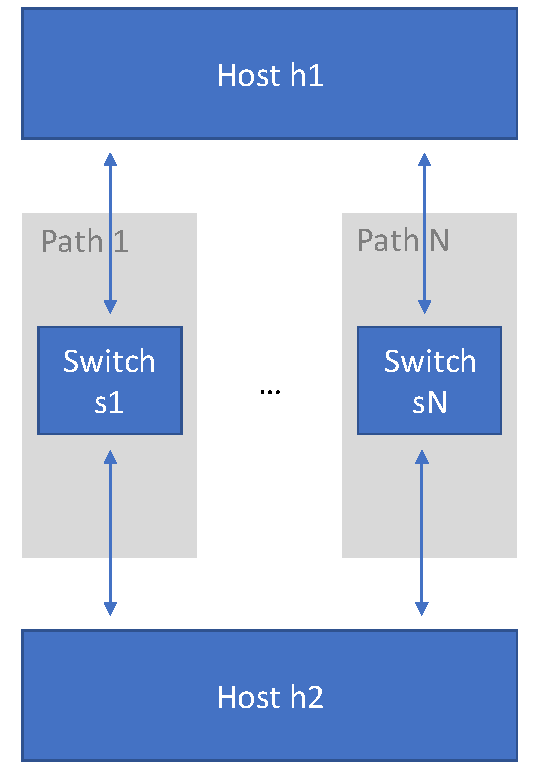
\includegraphics[width=0.3\textwidth, trim=3.5mm 1mm 3.5mm 1mm, clip]{mininet-structure.pdf}
	\caption{Structure of our Mininet networks}
	\label{fig:mininet-structure}
\end{wrapfigure}


As a virtual network environment, we use Mininet, ``a system for rapidly 
prototyping large networks on the constrained resources of a single laptop'' \cite{Lantz10Mininet}.
It allows us to run our regular client and server software inside a simulated environment by placing them in separate network namespaces, a feature of Linux lightweight virtualization of different network configurations on the same system. Virtual network devices are used to connect the namespaces to virtualized switches.
%There is also support for simulation of custom Ethernet switches and Software-Defined Networking controllers, which we don't use

We use an evaluation framework which automatically sets up networks based on a declarative Python script. The networks always have the same fundamental structure: two hosts are connected over a specified number of isolated links as shown in Figure \ref{fig:mininet-structure}.
In the script, the links can be configured with regards to bandwidth, delay, packet loss, and queue size. We can also set the Multipath TCP BACKUP flag for a link, or can specify a time after which the path is broken.
We also implemented scripts which are run in the two hosts after the network is set up, to start the web server on one host, run the web request measurement on the other, and collect the data afterwards.
In this setup, the hosts have no connection to the public internet, therefore all web page resources have to be served by the local web server.


%\todo{short intro to mininet}

%\todo{our setup with mininet}

%\todo{...}


\subsection{Real World Measurements}

To confirm the measurements we conducted in Mininet, we ran the same software on real hardware and real networks. For the server side, we used virtual machines located in the Frankfurt data centre of Amazon Web Services and in the Roubaix data centre of OVH. As clients, we used notebooks connected to the internet via Wi-Fi and DSL, via a Wi-Fi hotspot with VPN tunnelling, and via USB to a mobile phone with an LTE connection.\footnote{We were unable to use the university's internet connection directly as its Firewall blocks Multipath TCP connections.}

We implemented a tool to run repeated web request measurements with different parameters at the client and server. Using an SSH connection to the server, the tool controls the remote scheduler setting, and retrieves statistics and logfiles. To evaluate behaviour dependent on round trip times, it can add a variable delay to packets sent over specific network interfaces.


\section{TCP Small Queues}

If there is a stall below the TCP layer, the TCP small queues \cite{LwnTSQ} algorithm ensures not too much data gets buffered in the FIFOs of network interfaces, e.g. when an application sends data faster than the network interface card can relay it. To do this, the algorithm checks \code{sk_wmem_alloc}, a field of the socket struct in the kernel, which stores the amount of memory currently used for the send buffer. The default multipath scheduler in the Linux kernel declares a subflow as temporarily unavailable if the underlying TCP socket is throttled, as seen in Listing \ref{lst:mptcp_is_temp_unavailable}. When using RBS, the information if a subflow is throttled is available as the property \code{<subflow>.THROTTLED} and can be considered in the scheduling decision.

\begin{lstlisting}[style=C_Code,label=lst:mptcp_is_temp_unavailable,caption={Excerpt from Multipath TCP Kernel, \code{net/mptcp/mptcp_sched.c}
%\footnote{url{https://github.com/multipath-tcp/mptcp/blob/e076f6be0f4b3d48d59c686d0a9ff4b87bc91a0f/net/mptcp/mptcp\_sched.c\#L39}}
}]
static bool mptcp_is_temp_unavailable(struct sock *sk,
				      const struct sk_buff *skb,
				      bool zero_wnd_test)
{
 [...]
	/* If TSQ is already throttling us, do not send on this subflow. When
	 * TSQ gets cleared the subflow becomes eligible again.
	 */
	if (test_bit(TSQ_THROTTLED, &tp->tsq_flags))
		return true;
\end{lstlisting}

This is where a difference between simulated and real networks exists: in Mininet the TCP Small Queue throttling never got engaged, because \code{sk_wmem_alloc} never changes from its initial value of \code{1}. This is consequential, as the virtual ethernet devices don't have to really transmit any data, instead only passing along a pointer, and therefore never need to buffer it.

In our simulations, each packet is delayed in the network emulation (netem) layer, and traffic shaping is used, to simulate a real link with latency and limited bandwidth. This layer resides between the TCP stack and the virtual ethernet device, therefore it should cause \code{sk_wmem_alloc} to increase, but it didn't.
%-        Gilt das auch f�r shaping ohne delay, e.g., 10 Mbit bw? W�rde es ohne den patch also mit 10Mbit und ohne delay �wie erwartet� laufen?
When using only traffic shaping, but not the delaying functionality of netem, the problem does not occur. 

%https://kernelnewbies.org/Linux_3.6#head-b1e33c4c78affb4186e5affc4b4a2bc7d44a3e66
%https://lwn.net/Articles/507065/

So we built a test case where a delay is added on one host with netem\footnote{\code{tc qdisc add dev h1-eth0 root netem delay 5000ms}}, and then \code{iperf} is run to create traffic between the host. We also added a debug output to the function \code{tcp_small_queue_check} in \code{net/ipv4/tcp_output.c} \footnote{\url{http://lxr.free-electrons.com/source/net/ipv4/tcp_output.c\#L2074}} to see if TSQ will throttle the output. But in Mininet / veth, \code{sk_wmem_alloc} is always at the value \code{1}. The \code{TSQ_THROTTLED} never gets set. If doing the same on two machines connected over ethernet cable, \code{sk_wmem_alloc} raises, and eventually \code{TSQ_THROTTLED} is set.

An inquiry on the Mininet mailing list resulted\footnote{\url{https://mailman.stanford.edu/pipermail/mininet-discuss/2017-April/007425.html}} in the hint that the latency emulation code calls \code{skb_orphan_partial}, which reduces the socket buffer's size to \code{1}, therefore essentially removing it from \code{sk_wmem_alloc}.
This further lead us to a code comment in the Linux kernel which says that this behaviour is by design, because ``orphaning usually takes place at TX completion time, so \_before\_ the link transit delay'' (Linux kernel 4.4, \code{net/sched/sch_netem.c}, line 429). 
%-        Netem delay packets werden EXTRA rausgenommen, weil?
The reason is that the netem layer is designed to emulate delays in the \textit{network}, not \textit{network interface}, to test e.g. TCP congestion control algorithms. Therefore, it needs to behave as if the delay occurred after orphaning the socket buffer.  But we want do emulate delays in the \textit{network interface} in this case, so we change this behaviour by commenting out the call to \code{skb_orphan_partial} as shown in Listing \ref{lst:sch_netem}. To see if the call would have been normally made, we also added a debug output temporarily. This enabled us to test the TSQ throttling in our simulation with Mininet.


\begin{lstlisting}[style=RBS,label=lst:sch_netem,caption={Modified version of Linux kernel 4.4, \code{net/sched/sch_netem.c}, line 398ff},linebackgroundcolor={\lstLinesRemoved{13-14}\lstLinesAdded{16-18}}]
/*
 * Insert one skb into qdisc.
 * Note: parent depends on return value to account for queue length.
 *      NET_XMIT_DROP: queue length didn't change.
 *      NET_XMIT_SUCCESS: one skb was queued.
 */
static int netem_enqueue(struct sk_buff *skb, struct Qdisc *sch)
{
 [...]
        /* If a delay is expected, orphan the skb. (orphaning usually takes
         * place at TX completion time, so _before_ the link transit delay)
         */
        // if (q->latency || q->jitter)
        //         skb_orphan_partial(skb);

        printk("netem_enqueue: ...not calling skb_orphan_partial, "
               "latency=%ld, jitter=%ld, sk=%p, sk_wmem_alloc=%d", q->latency, q->jitter,
               skb->sk, skb->sk == NULL ? 0 : atomic_read(&skb->sk->sk_wmem_alloc));
\end{lstlisting}










\clearpage

\section{Evaluations}

In this section, we present the setup and results of three evaluations we conducted 
with schedulers which use application-provided hints.

\subsection{Evaluation A (``Bad Wi-Fi'')}
% zeigen - implementiertung funktioniert grunds�tzlich
% simple (``academic'') content-type specific scheduling


The goal of this evaluation is to test the implementation of content-type 
specific scheduling, and to show a first content-type based optimization of 
existing and modified web pages. The network situation is shown in Figure \ref
{eva1-scenario}. A user surfs the web on a smartphone which is connected to 
a free Wi-Fi hotspot and a cellular network. The Wi-Fi routes the traffic 
through a VPN and therefore incurs a high latency, but has acceptable 
bandwidth and no traffic limit. In contrast, the cellular network has low 
latency but a metered traffic limit and is therefore considered as ``
expensive''.
The scenario is emulated in Mininet. Client and server are modelled as 
Mininet hosts running the Google Chrome browser and the Nghttpd web server, 
respectively. They each have two interfaces, which are connected by two 
Mininet links with delay and rate limiting to simulate the two connection 
paths. 

The web pages we used are an unmodified article from CNN, and the original 
and a modified version of the English Wikipedia home page. They consist of an 
HTML document referencing style sheet, script and images of different size. 
On the Wikipedia page, all styles and scripts are included in the \code{<head>}
of the document and required for rendering the page. In the modified 
version, we included two big images below the fold that are not required for 
the rendering.

The scheduler script, which is listed in Annex B, was designed to send the images only over the ``cheap'' Wi-Fi
subflow, and allow the other, more time-critical data, to choose from the 
available subflows the one with the lowest round-trip time.
For comparison, we use two reference schedulers, one that is single path TCP 
equivalent as it only transmits on the non-backup subflow, and one 
``aggressive'' scheduler that ignores the backup flag and always uses the 
fastest available subflow.



%story:
% situation: unmetered wifi hotspot with high latency, metered cellular with low latency
% results:
%  without mptcp - using only slow wifi - firstMeaningfulPaint X sec, load X sec
%  without mptcp - using only cellular - fast, but expensive
%  with 'stupid' mptcp - min_rtt scheduler, using both paths - firstMeaningfulPaint X sec, load X sec, uses lots of cellular data volume
%		-> because cellular has lower rtt, equal to cell only -> fast, but expensive
%  with 'intelligent' mptcp - min_rtt scheduler, using cellular only for 'important' stuff - firstMeaningfulPaint X sec, load X sec,
%			uses not that much cellular data, firstMeaningfulPaint as fast as cell only, but load slower -> compromise ``cheap and (kinda) fast''




%sudo python2 execute.py --congestion_control cubic --network badWifiHotspot -a http2 --scheduler 'min_rtt_ctype_aware.txt min_rtt_advanced.txt'
%badwifi.ipynb


We run the simulation multiple times for every combination of scheduler, 
network and web page and look at the averaged received bytes per interface, 
as well as the browser timings. 

\begin{figure}[h]
\centering
	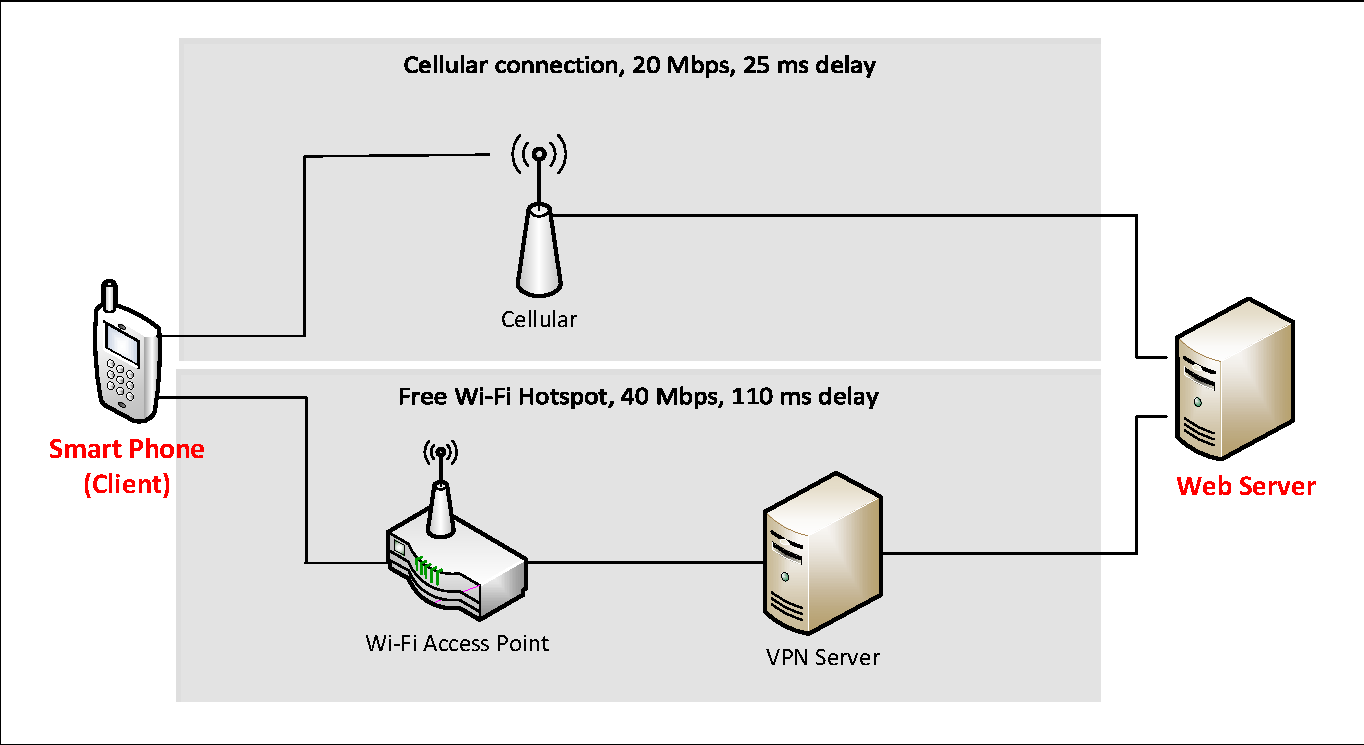
\includegraphics[width=0.9\textwidth]{eva1-scenario.pdf}
	\caption{Network scenario which is simulated in Evaluation A }
	\label{eva1-scenario}
\end{figure}


In figure \ref{eva1-loadtimes} the timing metrics are shown, grouped by page
and used scheduler. Comparing the results of using the content-aware scheduler 
and the aggressive reference scheduler, the time to first meaningful paint is 
the same, while saving a considerable amount of data volume on the cellular 
connection. 
Compared to using the high latency subflow as the only path, the
schedulers which use multiple paths are faster by multiple seconds.
For the CNN article, the data volume saved is 4.6 MB per page load as shown 
in figure \ref{eva1-rxbytes} and the speed up of the first meaningful 
paint event is from 4.5 to 2.8 seconds.

\begin{figure}[h]
\begin{center}
	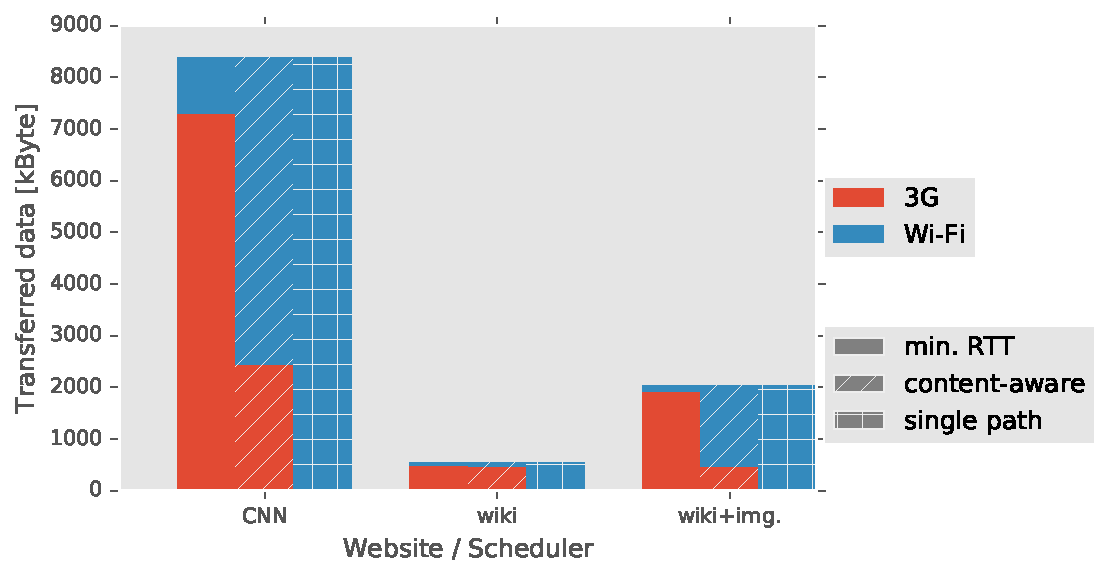
\includegraphics[width=0.9\textwidth]{eva1-rxbytes.pdf}
	\caption{Received bytes per interface for Evaluation A }
	\label{eva1-rxbytes}
\end{center}
\begin{center}
	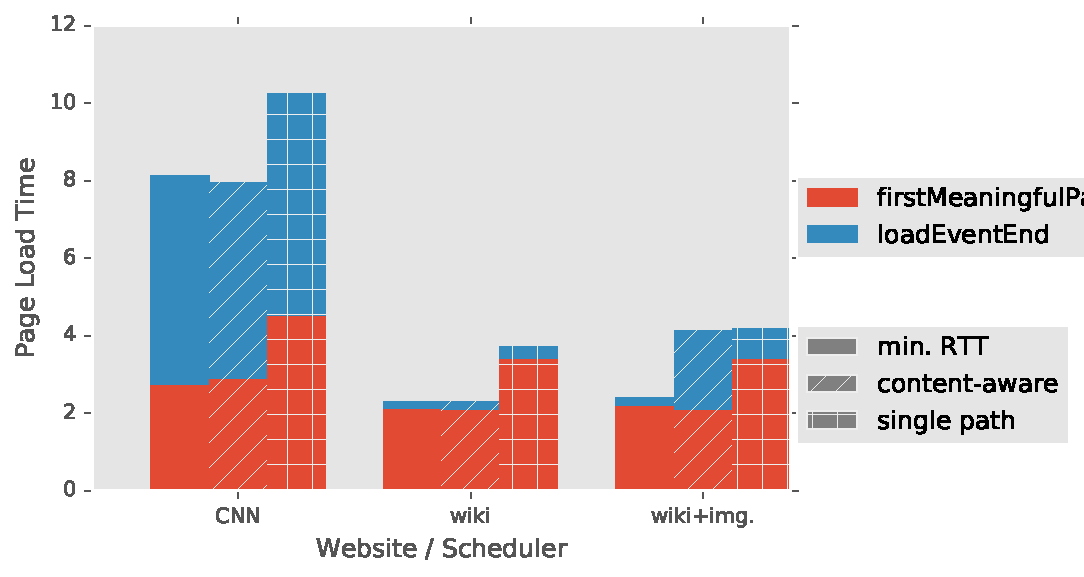
\includegraphics[width=0.9\textwidth]{eva1-loadtimes-stacked.pdf}
	\caption{Mean page load times for Evaluation A }
	\label{eva1-loadtimes}
\end{center}
\end{figure}



% simulated netw. with mininet
% - two hosts, two paths
% - path one (slow Wi-Fi hotspot, e.g. over vpn) - bw=50, delay=110
% - path two (LTE) - bw=50, delay=50
% server: nghttpd, modified for RBS socket options
% - hint: content type (document, style, script, image, other)
% scheduler: rbs
% - forTest: script 1: redundant for document+style
% - forTest: script 2: never transmit images on LTE
% baselines:
% - script 3: redundant scheduler (everything redundant)
% - linux mptcp default scheduler
% - single path tcp on Wi-Fi
% - single path tcp on LTE
% web site:
% - synthetic web site with:

% later ajax redundant
% oder images only one sbf


\clearpage

\subsection{Evaluation B (``Real World'')}


% subflow attributes
\begin{wraptable}{r}{9cm}
	\begin{tabularx}{\linewidth}{ l r r r r r } \toprule
	Path & Loss & Min RTT & Mean RTT & Max RTT & Mdev \\ \midrule

	Wi-Fi &	10\%  &  105ms & 148ms  &  398ms &  27ms \\
	LTE	 &	0\%	  &  25ms  &  97ms  &  634ms &  95ms \\

	\bottomrule
	\end{tabularx}
	\caption{Network characteristics for Evaluation B}
	\label{tab:eva2-net-ping}
\end{wraptable}



To try our implementation in a real network, we set up a network environment 
as described in Figure \ref{eva1-scenario}. Instead of a smartphone, we used 
a notebook running Ubuntu Linux with the custom RBS kernel. It has two 
independent internet uplinks: an LTE connection, using USB tethering over an 
Android phone connected to Telefonica network in Darmstadt, Germany; and a 
connection via a free Wi-Fi hotspot of the Freifunk project\footnote{\url{https://darmstadt.freifunk.net}}, 
which sends all traffic through a VPN 
tunnel and is connected over a residential VDSL connection. The VDSL 
connection has an average RTT of 100ms, when going through the hotspot VPN, 
RTT rises to 150ms. 
The server is a virtual machine in a data centre in Roubaix, France and runs 
Debian Linux with the same kernel as the notebook. 

In section \ref{relwork-mptcp-performance} we learned that LTE RTTs vary 
widely, this was confirmed by our ping tests as visible in Table \ref{tab:eva2-net-ping}. 
Therefore, we need to average our results over a larger number of 
measurements than in the virtual environment, where delay is fairly uniform.
 This is why we did fewer variations than before. We use the 
same set of schedulers as described in Evaluation A, but load only the 
modified Wikipedia homepage, as the LTE data volume we have available for 
testing is limited. 

Of 144 page loads, 12 failed and are removed from the results. The load fails result 
from bursty packet loss on the Wi-Fi connection.
We have 120 successful page loads left, which are shown in table 
\ref{tab:eva2-results}, grouped by scheduler. The mean is 
therefore calculated over 40 records each. The averaged first meaningful 
paint and page load times are presented in Figure \ref{eva2-loadtimes-stacked}.


\begin{figure}[h]
\centering
\begin{subfigure}{.5\textwidth}
\centering
	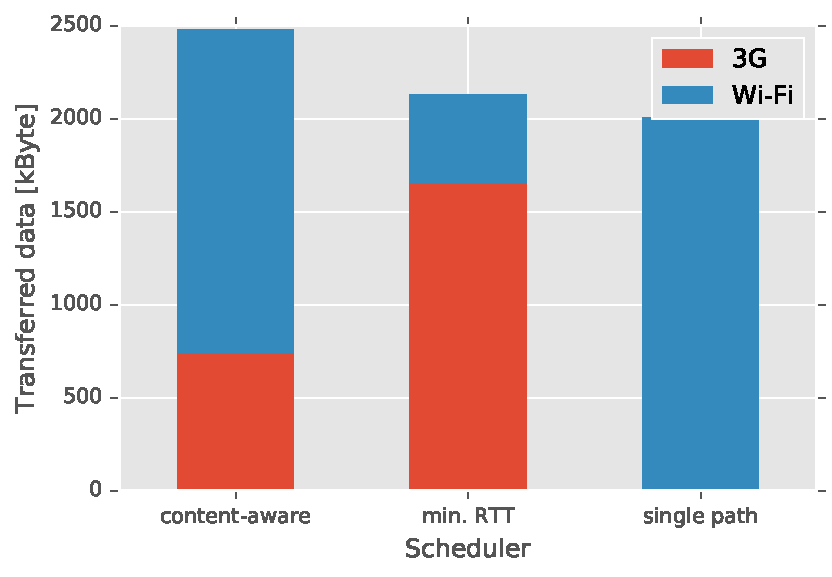
\includegraphics[width=\textwidth]{eva2-rxbytes.pdf}
	\caption{Received bytes per interface for Evaluation B }
	\label{eva2-rxbytes}
\end{subfigure}%
\begin{subfigure}{.5\textwidth}
\centering
	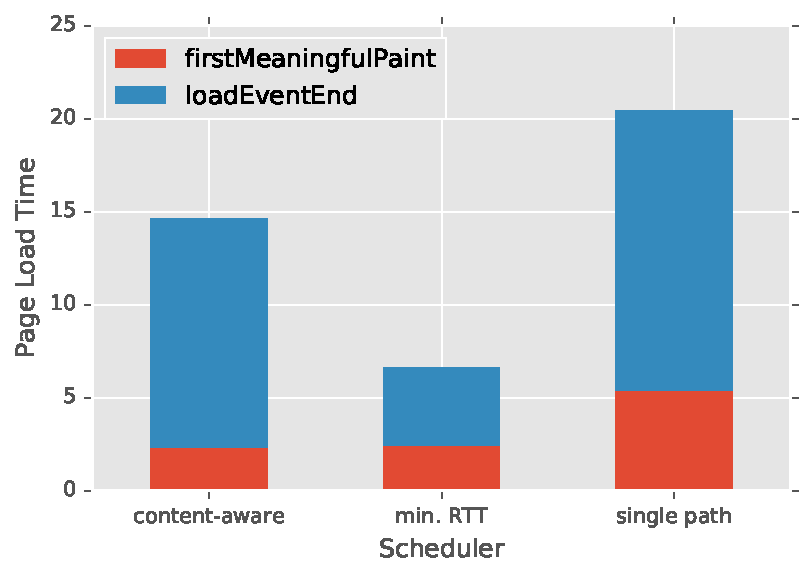
\includegraphics[width=\textwidth]{eva2-loadtimes-stacked.pdf}
	\caption{Mean page load times for Evaluation B }
	\label{eva2-loadtimes-stacked}
\end{subfigure}
\caption{Results of Evaluation B}
\label{fig:eva2}
\end{figure}

We see the performance of the content-aware scheduler
is approximately the same as the min. RTT scheduler for the user-perceived speed
as indicated by First Meaningful Paint times, which is almost more than 50\% faster
than single path performance. We also confirm the LTE bandwidth savings of the
content-aware scheduler when compared to the min. RTT scheduler, which are purchased
by higher page load times.
The results of these real-world measurements therefore confirm 
the findings of Evaluation A.




% subflow attributes
\begin{table}[t]
	\begin{tabularx}{\linewidth}{ l r r r r r } \toprule
Scheduler & Wi-Fi Data    &  LTE Data   &  DOM Content Loaded  &    First Meaningful Paint   &   Page Load Time \\ \midrule
      
  content-aware   &    1737.2 kB   &  740.7 kB  &   2.2 s &     2.2 s &    14.7 s   \\
  min. RTT     &   474.6 kB  &   1655.5 kB &    2.4 s   &  2.3 s    & 6.5 s \\   
  single path   &    1996.3 kB  &   1.5 kB  &   4.9 s   &  4.9 s   &  20.1 s  \\


	\bottomrule
	\end{tabularx}
	\caption{Aggregated measurement results for Evaluation B}
	\label{tab:eva2-results}
\end{table}


Furthermore, we want to check whether the ratio of Wi-Fi and LTE RTT affects 
the results. So, we add additional delays on the Wi-Fi channel. We compare the 
behaviour with 0ms, 8ms, 20ms and 85ms added one-way delay. We assume that, 
at least for the min. RTT scheduler, there should be a correlation of the RTT 
ratio and the amount of data offloaded to the 3G network, as offloading gets 
more ``attractive'' with higher Wi-Fi latency.

After running 10 page loads with each delay, however, we couldn't find such 
correlation with either scheduler. In Figure \ref{eva2-scat-rttRatio-dataRatio}
the fraction of data transmitted via LTE is plotted over the changing RTT 
ratio. All results for the single path scheduler we used for comparison are
at zero, so no data was sent over LTE, as expected. The single outlier could
be caused by measurement errors. 
The missing correlation could be caused by the fact that the min. RTT scheduler
itself doesn't have any notion of RTT ratio, but just saturates the congestion
window of the subflow with lowest RTT. The congestion window of the LTE connection
doesn't change with RTT ratio. Therefore, roughly the same amount of segments
``spill over'' to the slower Wi-Fi subflow.

\begin{figure}
\centering
	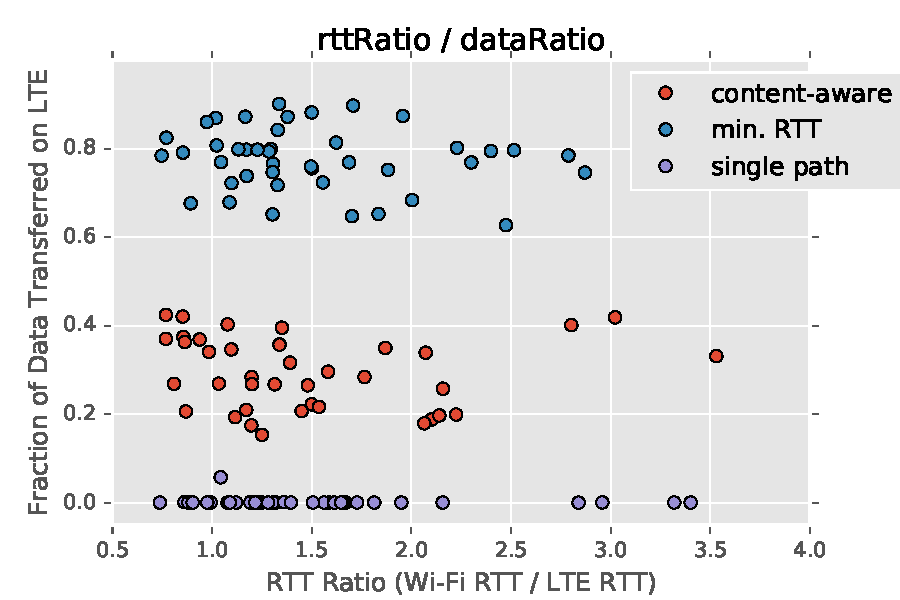
\includegraphics[width=0.7\textwidth]{eva2-scat-rttRatio-dataRatio.pdf}
	\caption{Subflow usage over RTT ratio for Evaluation B}
	\label{eva2-scat-rttRatio-dataRatio}
\end{figure}


\clearpage

When comparing Figure \ref{eva2-scat-rttRatio-firstMfPaint} and 
\ref{eva2-scat-rttRatio-loadEvent} we can see that the RTT ratio correlates
to paint and load timings in different ways for the three schedulers.
For single path operation, both get slower with rising RTT ratio, as the 
rising ratio means the Wi-Fi path gets slower (LTE stays roughly the same all 
the time).

The min. RTT scheduler just sends data over 3G when the Wi-Fi latency gets too
high, so the timings are don't change with the RTT ratio.
More interesting is the behaviour of the content-type aware scheduler, which is
not affected by RTT ratio in the First Meaningful Paint timing, as it behaves
like the min. RTT scheduler for the high priority data. But the Page Load Time
is affected, as the tail data can only be transmitted over the ``cheap'' Wi-Fi 
subflow.


\begin{figure}
\centering
\begin{subfigure}{.5\textwidth}
\centering
	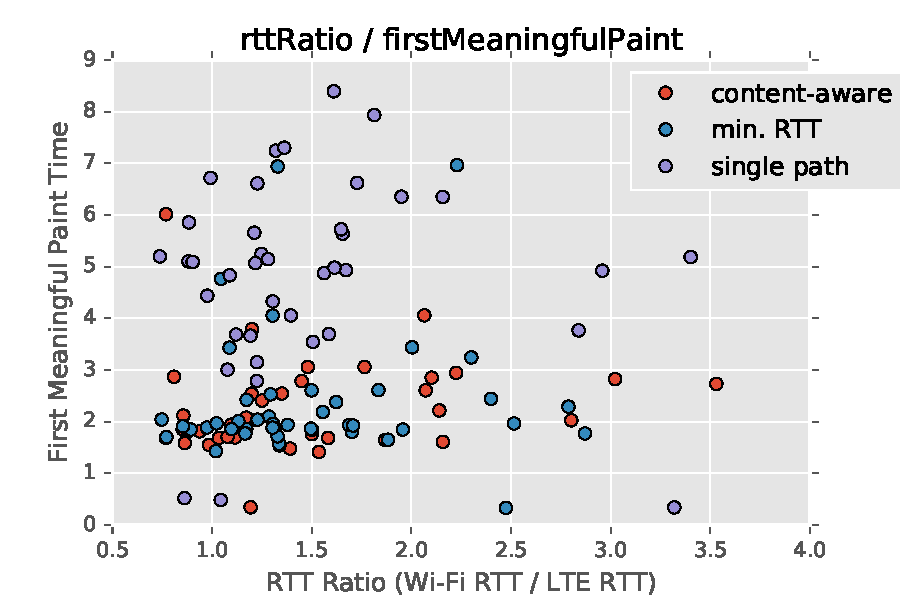
\includegraphics[width=\textwidth]{eva2-scat-rttRatio-firstMfPaint.pdf}
	\caption{First Meaningful Paint}
	\label{eva2-scat-rttRatio-firstMfPaint}
\end{subfigure}%
\begin{subfigure}{.5\textwidth}
\centering
	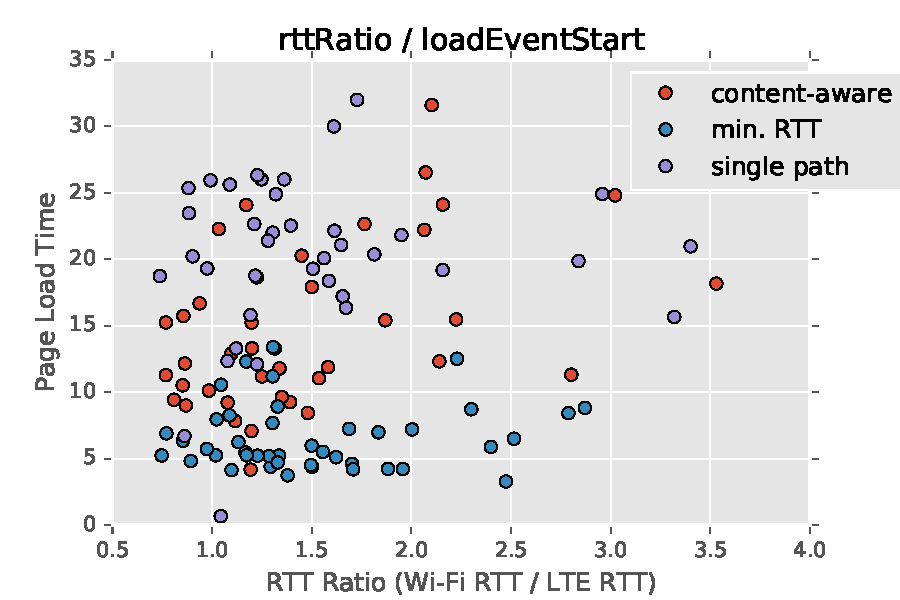
\includegraphics[width=\textwidth]{eva2-scat-rttRatio-loadEvent.pdf}
	\caption{Page Load Time}
	\label{eva2-scat-rttRatio-loadEvent}
\end{subfigure}
\caption{Page timings changing with RTT ratio for Evaluation B}
\label{fig:test}
\end{figure}









%wifi hotspot
%lte network of Telefonica in Darmstadt, Germany
%average LTE RTT of 60ms, Wifi of 140ms (?)


%However, as LTE has huge variation in RTT \textcite{Chen2013}, the bandwidth usage improvement of the content-aware scheduler in comparison to the minimal RTT scheduler are smaller in our real world evaluation.



\subsection{Evaluation C (``Lossy Wi-Fi'')}

We simulate a network with a similar scenario as Evaluation A, but now the 
Wi-Fi is faster than the LTE network in latency and bandwidth, but has a higher 
packet loss rate of 3\%. 
According to \textcite{Chen2013}, Wi-Fi has average loss rates from 1\% to 3\%,
while for LTE it is below 0.1\%. They also measured 30ms as average RTT for 
Wi-Fi, and at least 60ms for LTE, which we used for the simulation.

As an optimization for lossy networks we used a scheduler that redundantly sends
segments over all available subflows.
We could selectively enable this scheduler only if the packet loss raises above a 
defined threshold. 
Sending every packet twice will double the bandwidth usage,
but will also double the probability that at least one of the packets won't be lost,
guaranteeing ``that for every packet the
currently fastest path determines the effective end-to-
end latency'' \cite{Frommgen2016a}.

To conserve bandwidth, we only do redundant transmissions for 
latency critical data. For non-critical data, we transmit only on the fastest available
subflow. This content-aware scheduler is equivalent to switching between min. RTT and
redundant scheduler based on the content type. Its source code is reproduced in Annex C.
The application provides scheduling hints to help the scheduler decide whether the 
data is latency critical or not. We used the content type again as 
scheduling hints, and declared connection setup, main document, scripts and stylesheets
as latency critical. 
As reference schedulers, we used the same minimum round-trip time scheduler as in Evaluation A,
and additionally, a scheduler which sends all segments redundantly regardless of content type.

While simulating lossy networks, we noticed that for randomly distributed 
loss, the results can vary widely between page loads, depending on when 
during the connection packet loss occurs. This can be offset by repeating 
many times, and averaging the results. For the results presented below, we 
loaded the page 20 times with every scheduler.

The results are visualized in Figure \ref{eva3-rxbytes} and Figure \ref{eva3-loadtimes}.
In terms of data transmitted over LTE, the content-aware scheduler is again the 
compromise between the two references.
This is however offset by the fact that in this setup the used scheduler doesn't 
make any difference on the measured page paint and load times.
We also noticed that almost no data was transmitted on the Wi-Fi subflow. 
In total, only 8\% of the data was transmitted over Wi-Fi. 
We assume this is because after each loss, the Wi-Fi subflow is considered
congested, and will therefore often be not in the list of available subflows which have
free congestion window available. This would also explain why no difference in 
browsing speed was found.
It might be possible to change this by forcing non-critical traffic off the LTE
path by setting the multipath BACKUP flag on it.

Another possibility may be that losses didn't occur ``at the right moment'', especially
in the window when latency critical data is transferred. However, that is not too likely:
If we assume that 500 segments are transmitted redundantly with the content-aware scheduler, 
combined with a random packet loss of 3\%, the probability that at least one of the 
first 500 segments is dropped is over 99.9\%. 

Also, the ``ReMP TCP'' extension as proposed by \textcite{Frommgen2016a} has special
provisions for avoiding retransmissions of segments which were received on one path but
lost on the other. However, we couldn't recreate this behaviour in our RBS script, which
might be another reason for the missing performance benefit of the redundancy.


%\subsection{Evaluation D (``Lossy Wi-Fi'') (TODO!)}


\begin{figure}
\centering
	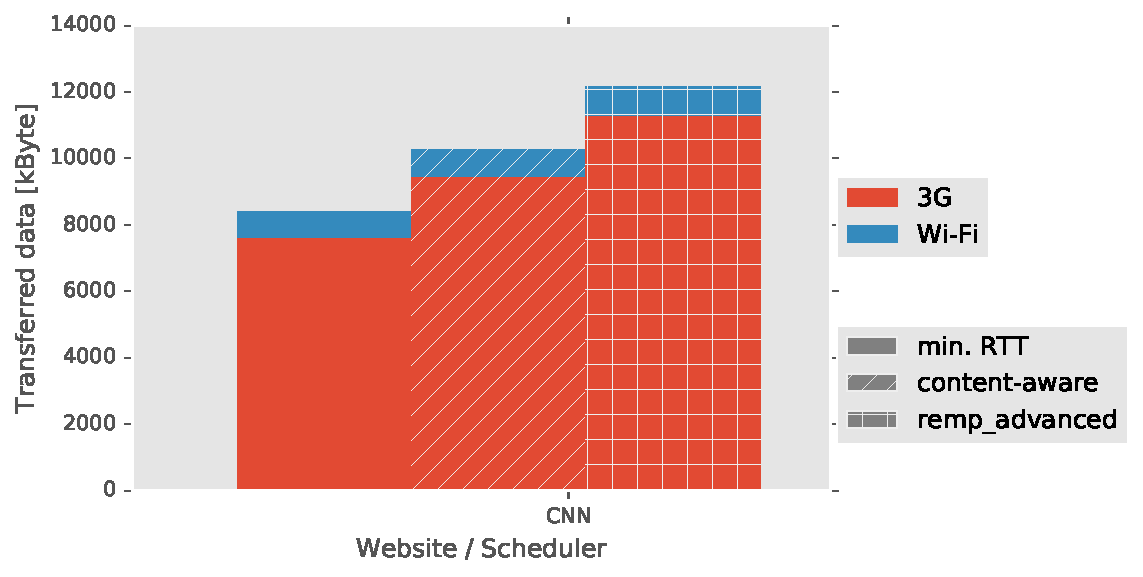
\includegraphics[width=0.7\textwidth]{eva3-rxbytes.pdf}
	\caption{Transferred data per subflow, for different schedulers, for Evaluation C}
	\label{eva3-rxbytes}
\end{figure}


\begin{figure}
\centering
	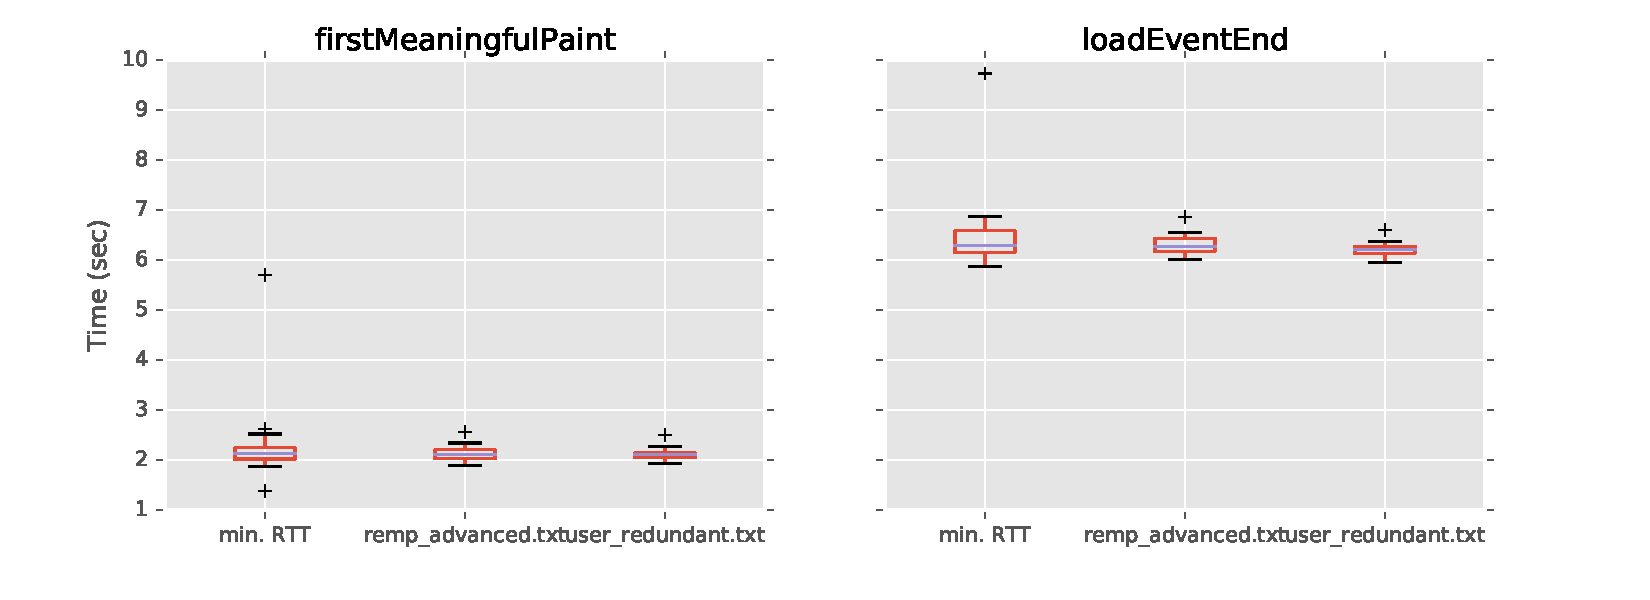
\includegraphics[width=\textwidth]{eva3-loadtimes.pdf}
	\caption{Timing metrics for different schedulers for Evaluation C}
	\label{eva3-loadtimes}
\end{figure}





%\todo{TODO}

%maybe redundant for ``important'' stuff?
% ...combination, switch dependent on RTT and LOSS -- maybe do this in a separate Eval C


%what could be done:
%try it over a real lossy network or over a simulation with better simulated loss




%\subsection{Evaluation C (``Combined'') (TODO!)}
%\todo{TODO}








%=====================================================================
\chapter{Conclusion}
%=====================================================================

As the main result from our work, we found that multipath scheduling can profit from hints from the application.
We found an exemplary network situation where the benefit is evident, as a performance improvement can be shown while minimizing additional data transfer costs. 
In evaluations A and B, we show speed-ups of 50\% compared to single path TCP by offloading segments to a faster, but more expensive subflow. To achieve this, only 34\% of the data needs to be transmitted on the more expensive subflow with the content-aware scheduler, instead of 75\% with the non-content-aware reference scheduler. Therefore we halve the loading time with only 45\% of the extra cost.


Based on the Nghttpd reference web server, we implemented cooperation of an application with the transport layer, and provide scheduler scripts to make use of scheduling hints passed by the server, allowing further experimentation with content-aware and other cooperative schedulers.
To make cooperation-based scheduling more generally applicable, we need to select different scheduling algorithms depending on the network conditions. 
In certain network scenarios, for example when available links are very heterogeneous, content-aware scheduling can make a difference in user-perceived performance. 

%\todo{conclusion}

\section{Outlook / Future Work}

Below we point out possible approaches for future investigations in the field of application-aware multipath scheduling, including further evaluations and development necessary for practical application.

%-------------------------------------------------------
%client side

The scheduler on the client side of optimizations was mostly excluded from our considerations. 
% one might implement a mptcp protocol extension so the logic can sit mostly in browser OR webserver, and the other side is instructed what to do
One could implement an MPTCP protocol extension allowing scheduling hints to be passed on over the network, so the cooperating application can be located in either the browser or the web server, while on the other side no application changes are needed.
% another way to generalize this could be definining a way for the web page/app to give the hints to the browser, which passes them on to the client mptcp scheduler
Another idea for generalization is to define an interface for the web page to give hints about the priority of the request to the browser, which would pass them on to the client MPTCP scheduler, which could even in turn forward them via above mentioned extension.
This could be especially interesting for AJAX requests, as their latency requirements can range from user-interactive, over regularly updating data, down to invisible background requests for which completing eventually is enough.
% -> the server scheduler implementation could send the corresponding mptcp frames with the same scheduling strategy as the request

% on the other hand, a different, quite simple approach could be taken on the browser side: send regular GET requests (maybe also POST with small body) as fast, latency critical strategy, while sending big POSTs (uploads) as latency uncritical strategy
On the other hand, a quite simple approach could be evaluated on the browser side: sending regular GET requests with a ``fast'' strategy, while choosing a bandwidth conserving strategy for POST requests, which often are big uploads.
% it might be possible to do a good heuristical approach here, without support from the browser, only in the mptcp scheduler
A heuristical approach without support from the browser might be good enough.

%-------------------------------------------------------
%we only ran a single page load in our evaluations
In our evaluations, we only performed single page loads. One could look at the behavior for further loads, when the MPTCP, TLS and HTTP2 connection is already established. Again, dynamic sites which use AJAX requests could be interesting test objects for further measurements.
% one could look at the behavior for further loads, when the MPTCP/TLS/HTTP2 connection is already established
% also, dynamic sites use xhr requests after they have load - these can be performance critical (e.g. if triggered by user interaction and results should be displayed) or less so (e.g. tracking user clicks, or refresh stuff regularly in the background) 
Furthermore, we only modified scheduling, but don't modify or block any resources, so the that web site is not changed or rendered unusable. Combining a compressing proxy or an ad blocker on the user side, can outweigh performance and 


%-------------------------------------------------------
%more interfaces

% ***Extension to three or more interfaces
%\todo{Extension to three or more interfaces}
Another area is extending the evaluations to three or more interfaces, and to multiple interfaces at the server, possibly allowing full meshed subflows.
%-------------------------------------------------------
%automated web site analysis
% ***our work could be combined with :
Some optimizations rely on manually providing resource priorities and dependencies to the web server. Our work could be combined with automated algorithms to determine dependency graphs of web pages and user relevancy ratings of resources as proposed by \textcite{klotski2015}.
% - automated categorization of ressources/http requests
%\todo{...}
% - automated dependency graph
%Automatische Einstufung von Seitenbestandteilen (HTTP Requests) in Relevanz / User Utility
%-> nicht Thema der Arbeit, aber evtl. relevant f�r praktische Umsetzung
%Automatisches Aufbauen von Dependency Graphs
%-------------------------------------------------------
%real web server
% ***Porting to a ``real'' web server e.g. apache or nginx
%\todo{Porting to a ``real'' web server e.g. apache or nginx}
Finally, to use the optimizations in a real-world scenario, it is necessary to port our modifications to Nghttpd to a ``real'' web server like Apache HTTP Server or Nginx.


%=====================================================================
% Bibliography
%=====================================================================


%\nocite{*}
%\chapter{Bibliography}
%\bibliography{thesis-h2-mptcp}{}
\pdfbookmark[0]{Bibliography}{Bibliography}
\printbibliography


\begin{appendices}

%\chapter{Web Request Measurement Script}\label{annex-measure_web_requests}

%\lstinputlisting[language=Python,caption={
%\code{measure_web_requests.py}
%}]{measure_web_requests.py}


\chapter{Content Type Detection Code}\label{annex-prepare_response}

\begin{lstlisting}[style=C_Code,caption={
\code{HttpServer.cc}, function \code{prepare_response}
}]
void prepare_response(Stream *stream, Http2Handler *hd, bool allow_push = true) {
  [...]
  auto query_pos = std::find(std::begin(reqpath), std::end(reqpath), '?');
  if (query_pos != std::end(reqpath)) {
    [...]
    const char* pos=(char*)query_pos;
    while(*pos!='\0') {
      if (*pos != '&' && *pos != '?') break;        pos++;
      // set multipath tcp scheduler register
      if (strncmp("rbs_set_R",pos,9)==0) {          pos+=9;
        int regnum = strtol(pos, (char**)&pos, 10);
        if (*pos != '=') break;                     pos++;
        int regval = strtol(pos, (char**)&pos, 0);
        if (regnum < 1 || regnum > 6) break;
        hd->set_rbs_register(regnum, regval);
      } else if (strncmp("rbs_user=",pos,9)==0) {   pos+=9;
        int regval = strtol(pos, (char**)&pos, 0);
        stream->priority_file_type = regval;
      }
    }
    raw_path = StringRef{std::begin(reqpath), query_pos};
    raw_query = StringRef{query_pos, std::end(reqpath)};
  } else {
    raw_path = reqpath;
  }
  [...]
  auto ext = file_path.c_str() + file_path.size() - 1;
  for (; file_path.c_str() < ext && *ext != '.' && *ext != '/'; --ext) ;
  if (*ext == '.') {
    ++ext;
    // only set content type if it was not overwritten by GET parameter earlier in this function
    if (stream->priority_file_type == 0) {
      // primitive file type categorization for scheduling
      if (!strcasecmp(ext, "jpg") || !strcasecmp(ext, "png") || !strcasecmp(ext, "gif")) {
        stream->priority_file_type = SKB_CONTENT_IMAGE;
      } else if (!strcmp(ext, "js")) {
        stream->priority_file_type = SKB_CONTENT_SCRIPT;
      } else if (!strcmp(ext, "css") || !strcmp(ext, "woff") || !strcmp(ext, "woff2")) {
        stream->priority_file_type = SKB_CONTENT_STYLE;
      } else if (!strcmp(ext, "html") || !strcmp(ext, "htm")) {
        stream->priority_file_type = SKB_CONTENT_DOCUMENT;
      } else {
        stream->priority_file_type = SKB_CONTENT_OTHER;
      }
    }
  }
  [...]
  hd->submit_file_response(StringRef::from_lit("200"), stream, file_ent->mtime,
                           file_ent->length, file_ent->content_type, &data_prd);
}
\end{lstlisting}





\chapter{Content Type and Cost Aware Scheduler}\label{annex-sched_eval_a}

\begin{lstlisting}[style=RBS,label=lst:sched_eval_a,caption={RBS Scheduler Script for Evaluation A and B},numbers=left]
/*
 * This scheduler sends packets on the subflow with the lowest RTT which has congestion window available
 *  ... except images, they are sent only on the "cheap" (non-backup) subflow (e.g. Wi-Fi instead of 3G)
*/
SCHEDULER min_rtt_ctype_aware;

VAR SKB_CONTENT_NOSTREAM = 1;
VAR SKB_CONTENT_DOCUMENT = 2;
VAR SKB_CONTENT_SCRIPT   = 3;
VAR SKB_CONTENT_STYLE    = 4;
VAR SKB_CONTENT_IMAGE    = 5;
VAR SKB_CONTENT_OTHER    = 6;

/* only use subflows which have CWND left*/
VAR usableSbfs = SUBFLOWS.FILTER(sbf => sbf.CWND > sbf.SKBS_IN_FLIGHT);

/* no subflows available? do nothing. */
IF (usableSbfs.EMPTY) { RETURN; }

/* send packets from resend buffer redundantly on the fastest new subflows */
IF (!RQ.EMPTY) {
	usableSbfs.FILTER(sbf => !RQ.TOP.SENT_ON(sbf)).MIN(sbf => sbf.RTT).PUSH(RQ.POP());
	RETURN;
}

IF (!Q.EMPTY) {
	/* simplified content type is passed along by the web server */
	VAR content_type = Q.TOP.USER;

	IF (Q.TOP.USER >= SKB_CONTENT_IMAGE) {
		/* the subflows marked as "BACKUP" are filtered out */
		usableSbfs.FILTER(sbf => !sbf.IS_BACKUP).MIN(sbf => sbf.RTT).PUSH(Q.POP());
	} ELSE {
		usableSbfs.MIN(sbf => sbf.RTT).PUSH(Q.POP());
	}
}
\end{lstlisting}

\chapter{Content-Based Redundant Scheduler}\label{annex-sched_eval_b}

\begin{lstlisting}[style=RBS,label=lst:sched_eval_b,caption={RBS Scheduler Script for Evaluation C},numbers=left]
/*
 * send packets redundant if skb user property is set
*/

SCHEDULER user_redundant;

VAR SKB_CONTENT_NOSTREAM =  1;
VAR SKB_CONTENT_DOCUMENT =  2;
VAR SKB_CONTENT_SCRIPT =    3;
VAR SKB_CONTENT_STYLE =     4;
VAR SKB_CONTENT_IMAGE =     5;
VAR SKB_CONTENT_OTHER =     6;

/* only use subflows which have CWND left*/
VAR usableSbfs = SUBFLOWS.FILTER(sbf => sbf.CWND > sbf.SKBS_IN_FLIGHT);

IF (usableSbfs.EMPTY) {
    RETURN;
}

/* send packets from resend buffer */
IF (!RQ.EMPTY) {
	/* is the user property set to "1"? -> important packet, send redundant */
	VAR notSentOnSbfs = usableSbfs.FILTER(sbf => !RQ.TOP.SENT_ON(sbf));
	IF (!notSentOnSbfs.EMPTY) {
		IF (Q.TOP.USER <= SKB_CONTENT_STYLE) {
			FOREACH(VAR sbf IN notSentOnSbfs) {
				sbf.PUSH(RQ.TOP);
			}
			DROP(RQ.POP());
		} ELSE {
			notSentOnSbfs.MIN(sbf => sbf.RTT).PUSH(RQ.POP());
		}
		RETURN;
	}
}

IF (!Q.EMPTY) {
	/* is the user property set to "1"? -> important packet, send redundant*/
	IF (Q.TOP.USER <= SKB_CONTENT_STYLE) {
		FOREACH(VAR sbf IN usableSbfs) {
			sbf.PUSH(Q.TOP);
		}
		DROP(Q.POP());
	} ELSE {
		usableSbfs.MIN(sbf => sbf.RTT).PUSH(Q.POP());
	}
}
\end{lstlisting}





\end{appendices}



\end{document}
